This section listed the plots that will be included in the paper. All the discussions are already covered in the results section. For the purpose of story telling, different panels are re-organized to be shown in the same plot.

\subsection{2-particle cumulant $v_n\{2\}$ with $n=2,3,4$}

\begin{figure}[H]
\centering
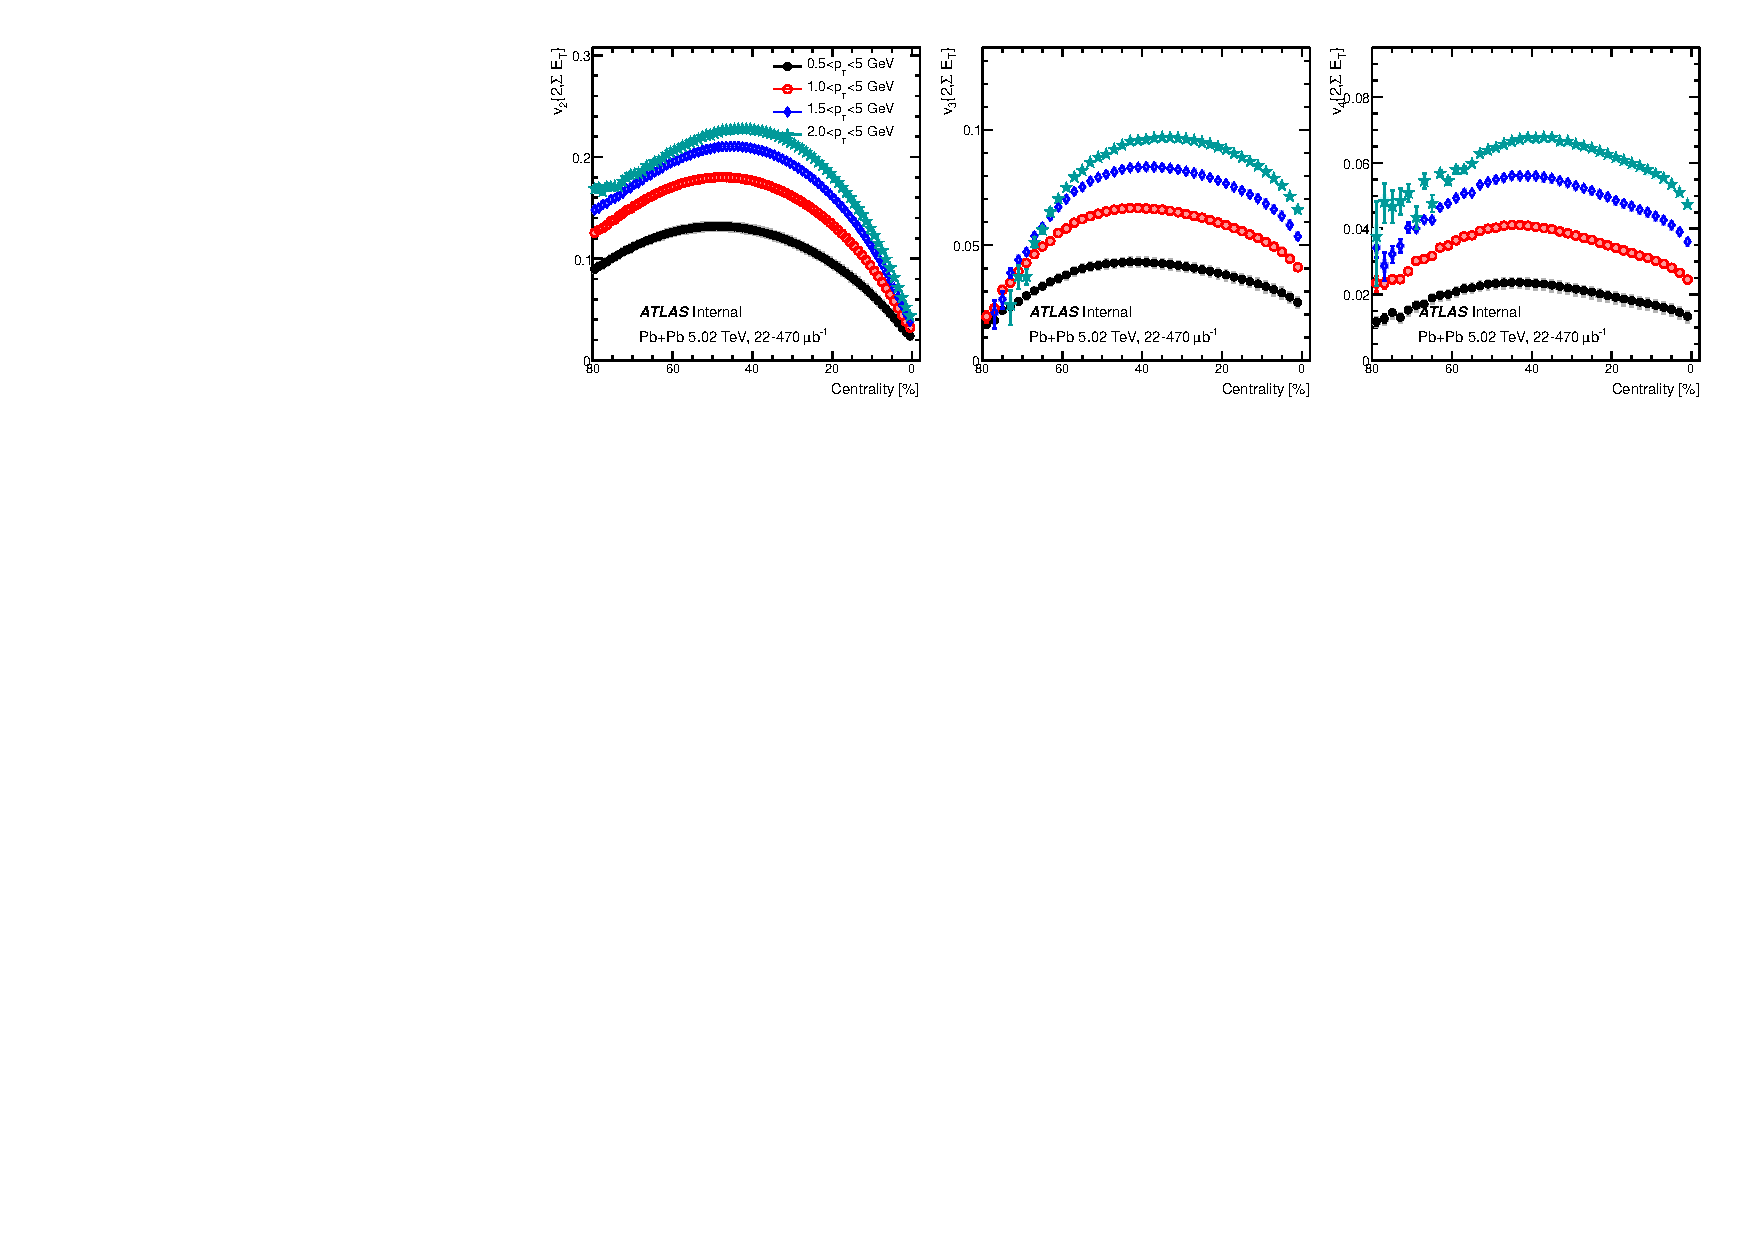
\includegraphics[width=.96\linewidth]{figs/sec_paper/comp_vn2_Cent.pdf}
\caption{2-particle flow cumulant as a function of centrality, calculated using standard method, with multiple $p_\text{T}$ ranges.}
\label{fig:paper_v2}
\end{figure}

\subsection{4-particle cumulant $nc_n\{4\}$ with $n=2,3,4$}

\begin{figure}[H]
\centering
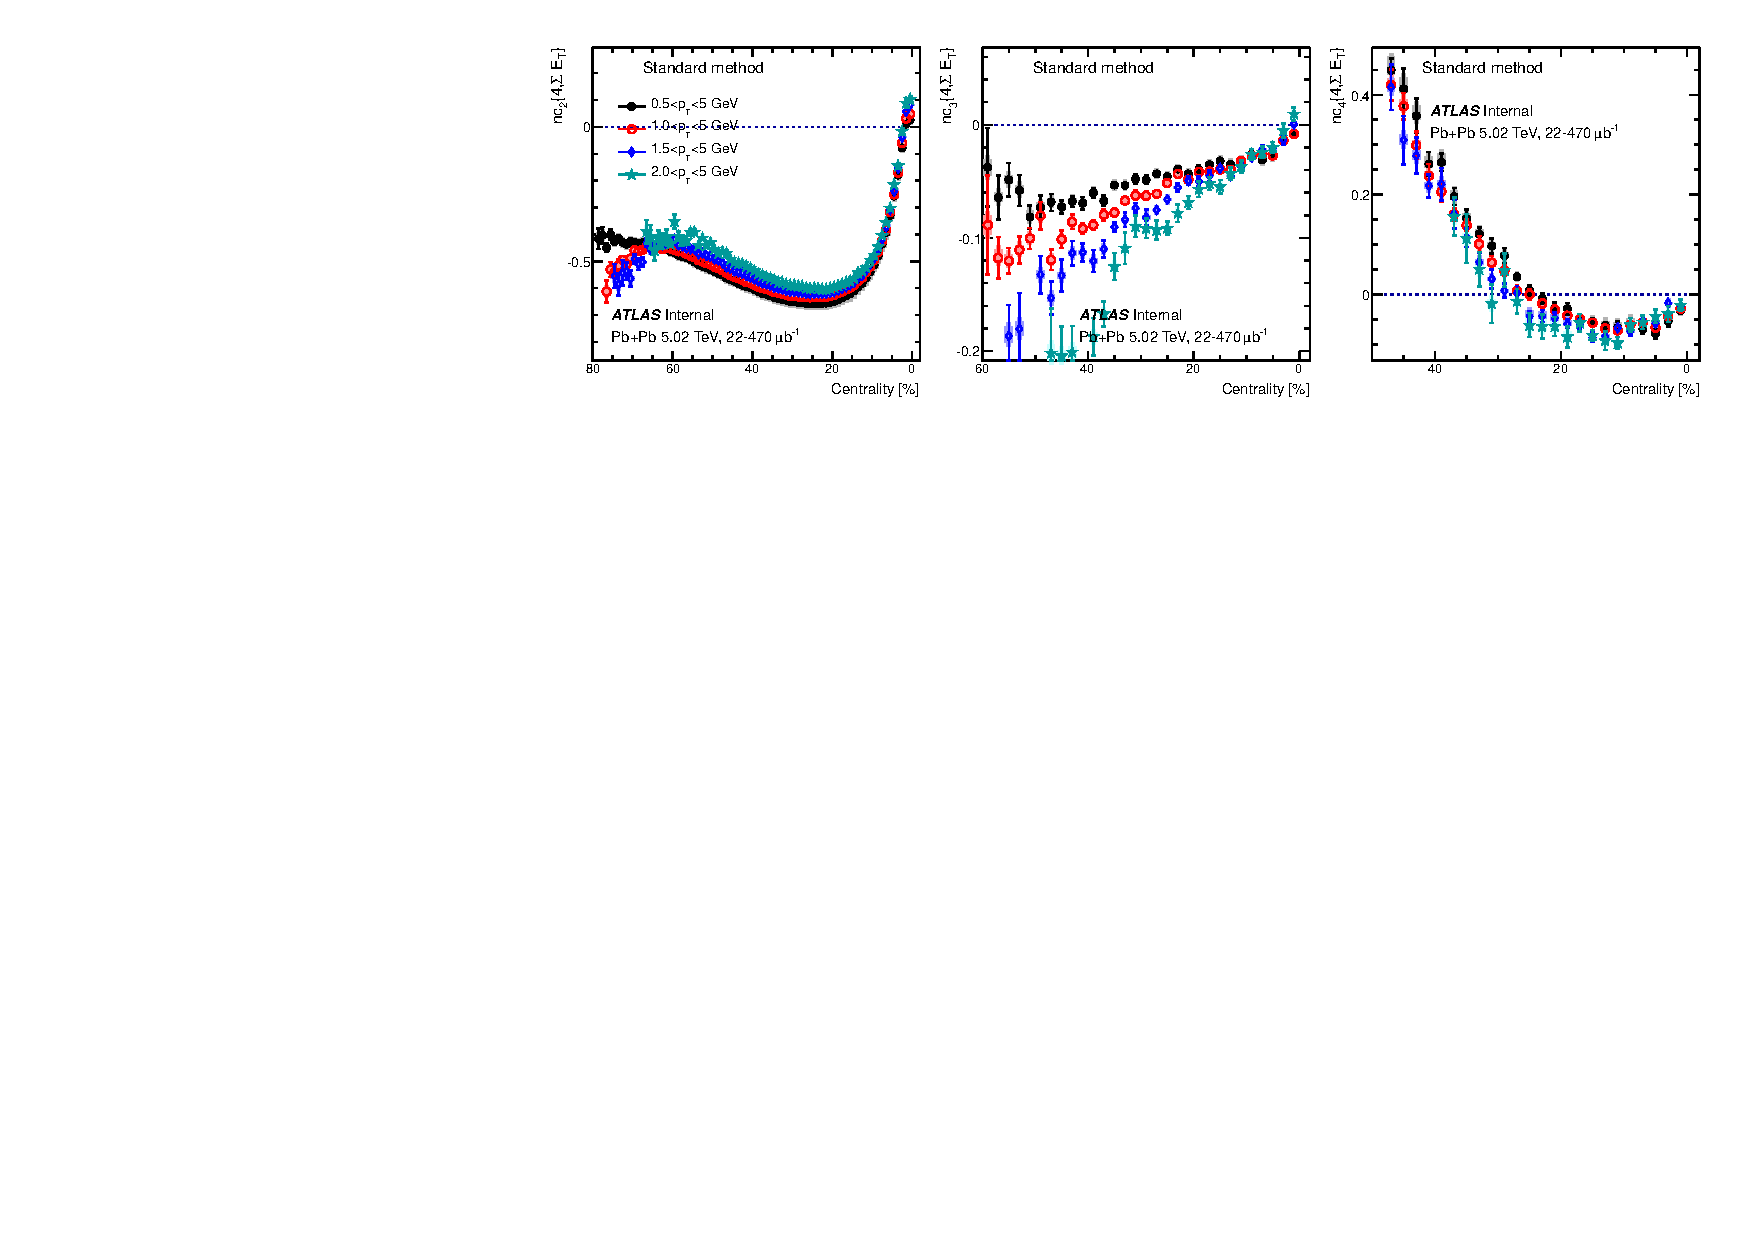
\includegraphics[width=.96\linewidth]{figs/sec_paper/comp_nc4_Cent.pdf}
\caption{4-particle normalized cumulant as a function of centrality, calculated using standard method, with multiple $p_\text{T}$ ranges.}
\label{fig:paper_nc4}
\end{figure}

\subsection{6-particle cumulant $nc_n\{6\}$ with $n=2,3,4$}

\begin{figure}[H]
\centering
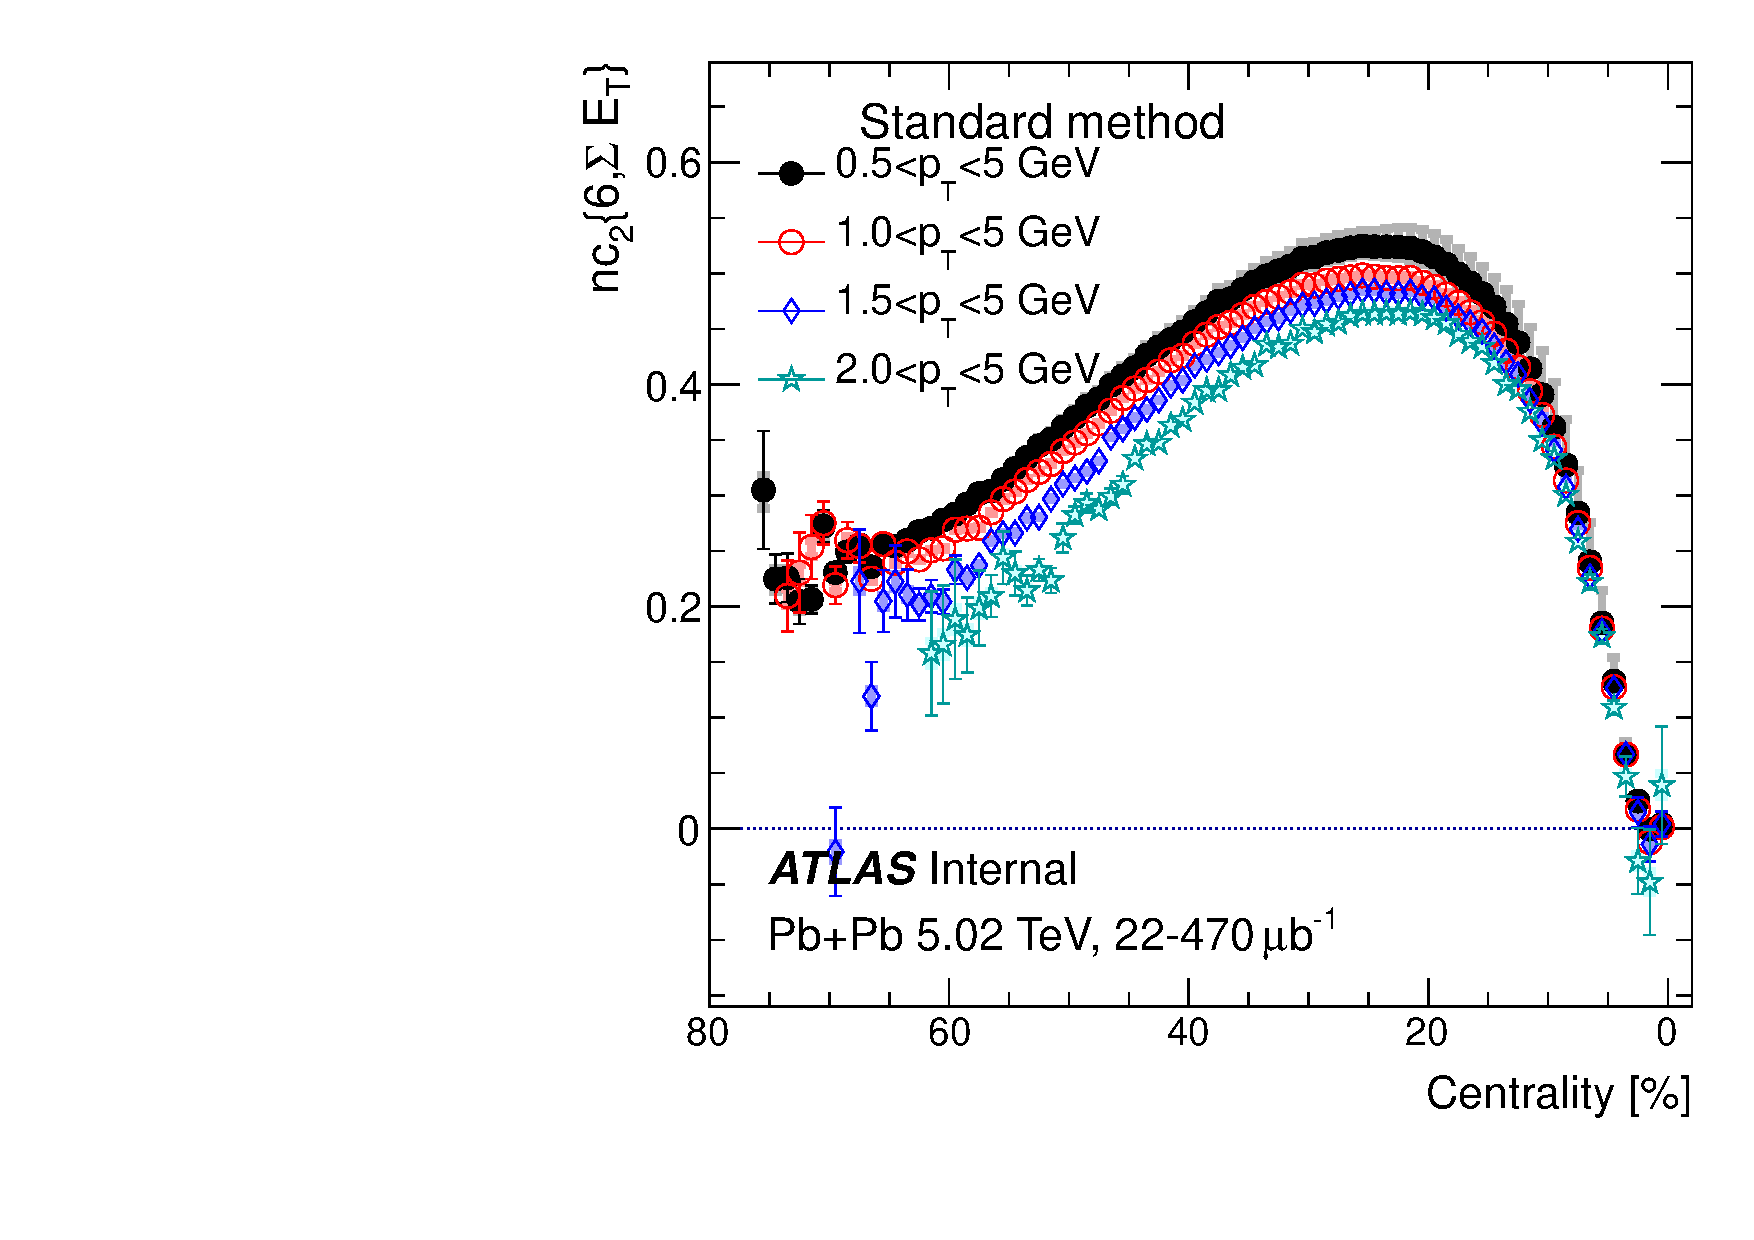
\includegraphics[width=.32\linewidth]{figs/sec_paper/comp_nc6_har2_Cent.pdf}
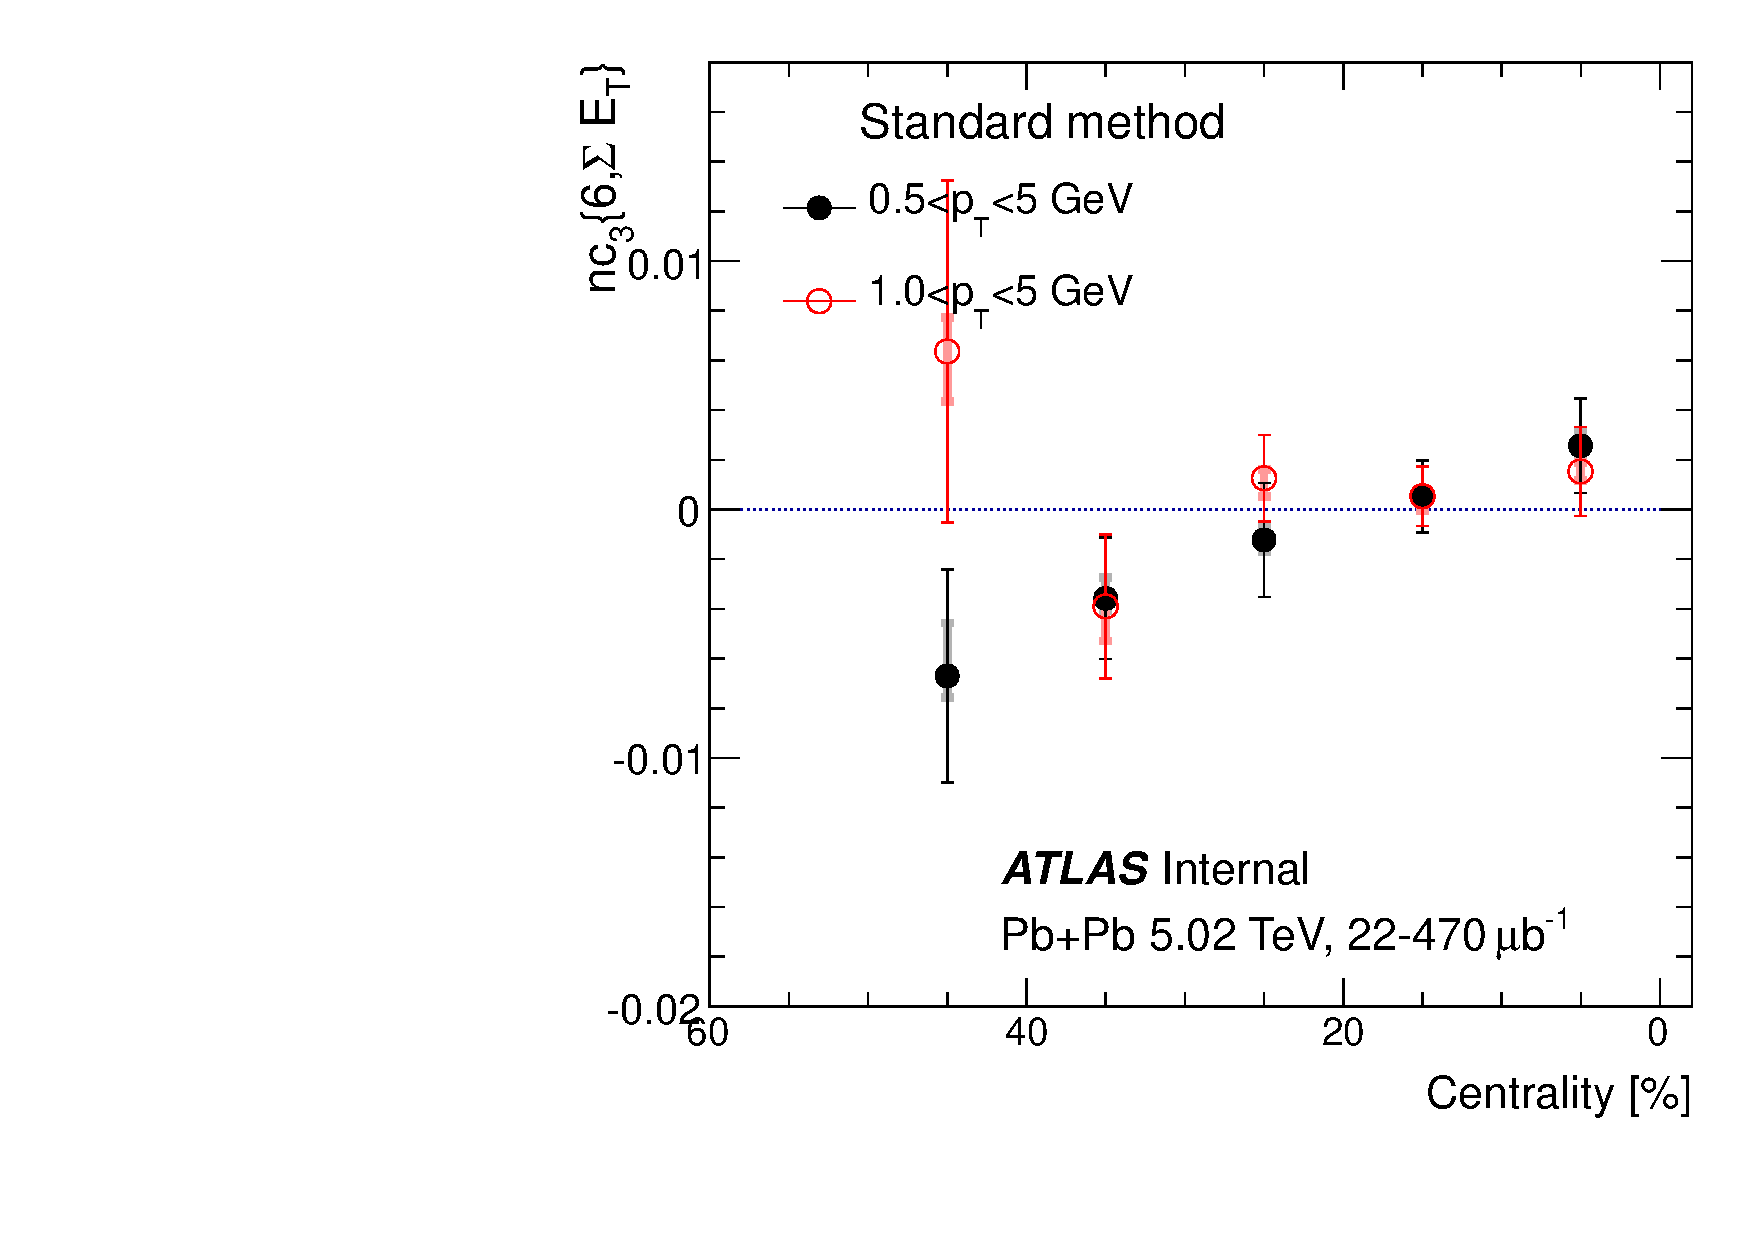
\includegraphics[width=.32\linewidth]{figs/sec_paper/comp_nc6_har3_Cent.pdf}
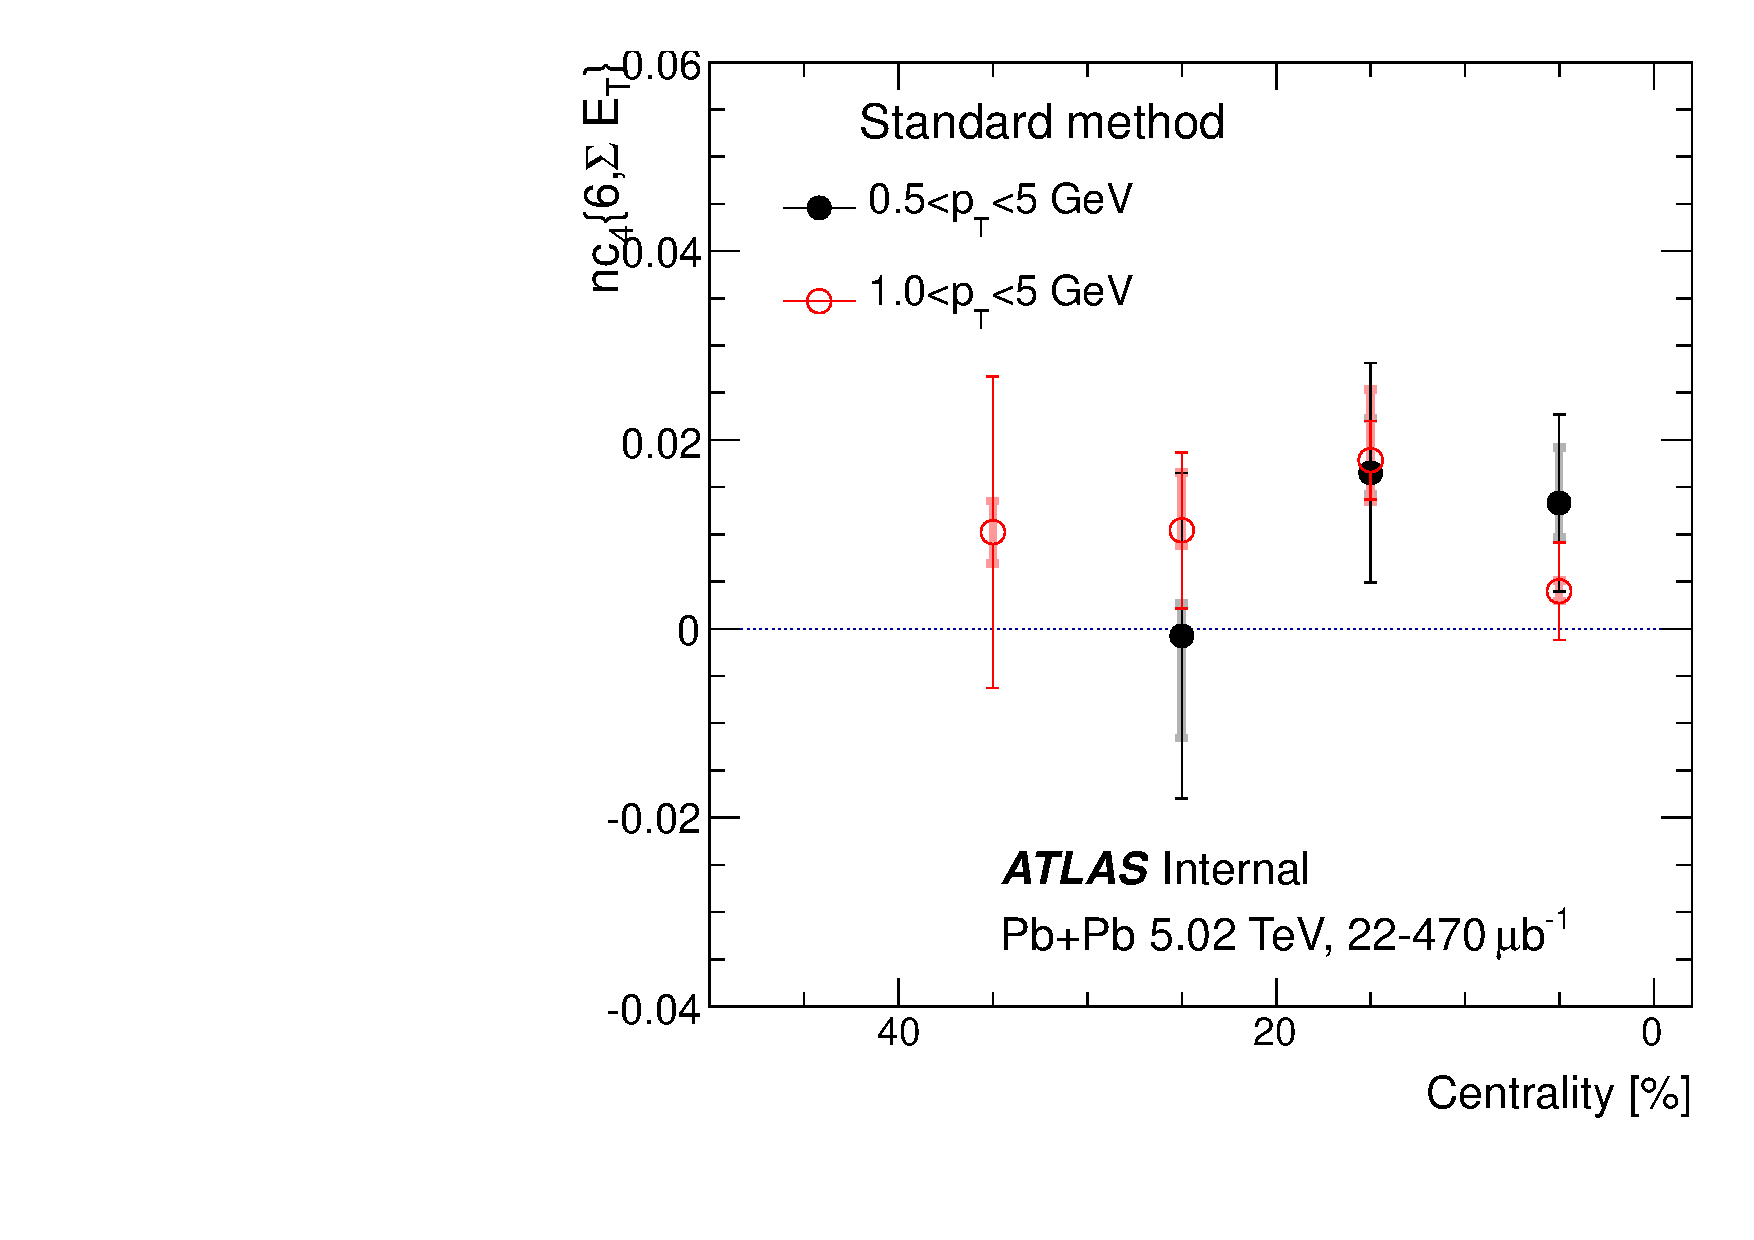
\includegraphics[width=.32\linewidth]{figs/sec_paper/comp_nc6_har4_Cent.pdf}
\caption{6-particle normalized cumulant as a function of centrality, calculated using standard method, with multiple $p_\text{T}$ ranges.}
\label{fig:paper_nc6}
\end{figure}

\subsection{Cumulant ratio $v_n\{4\}/v_n\{2\}$ with $n=2,3,4$}

\begin{figure}[H]
\centering
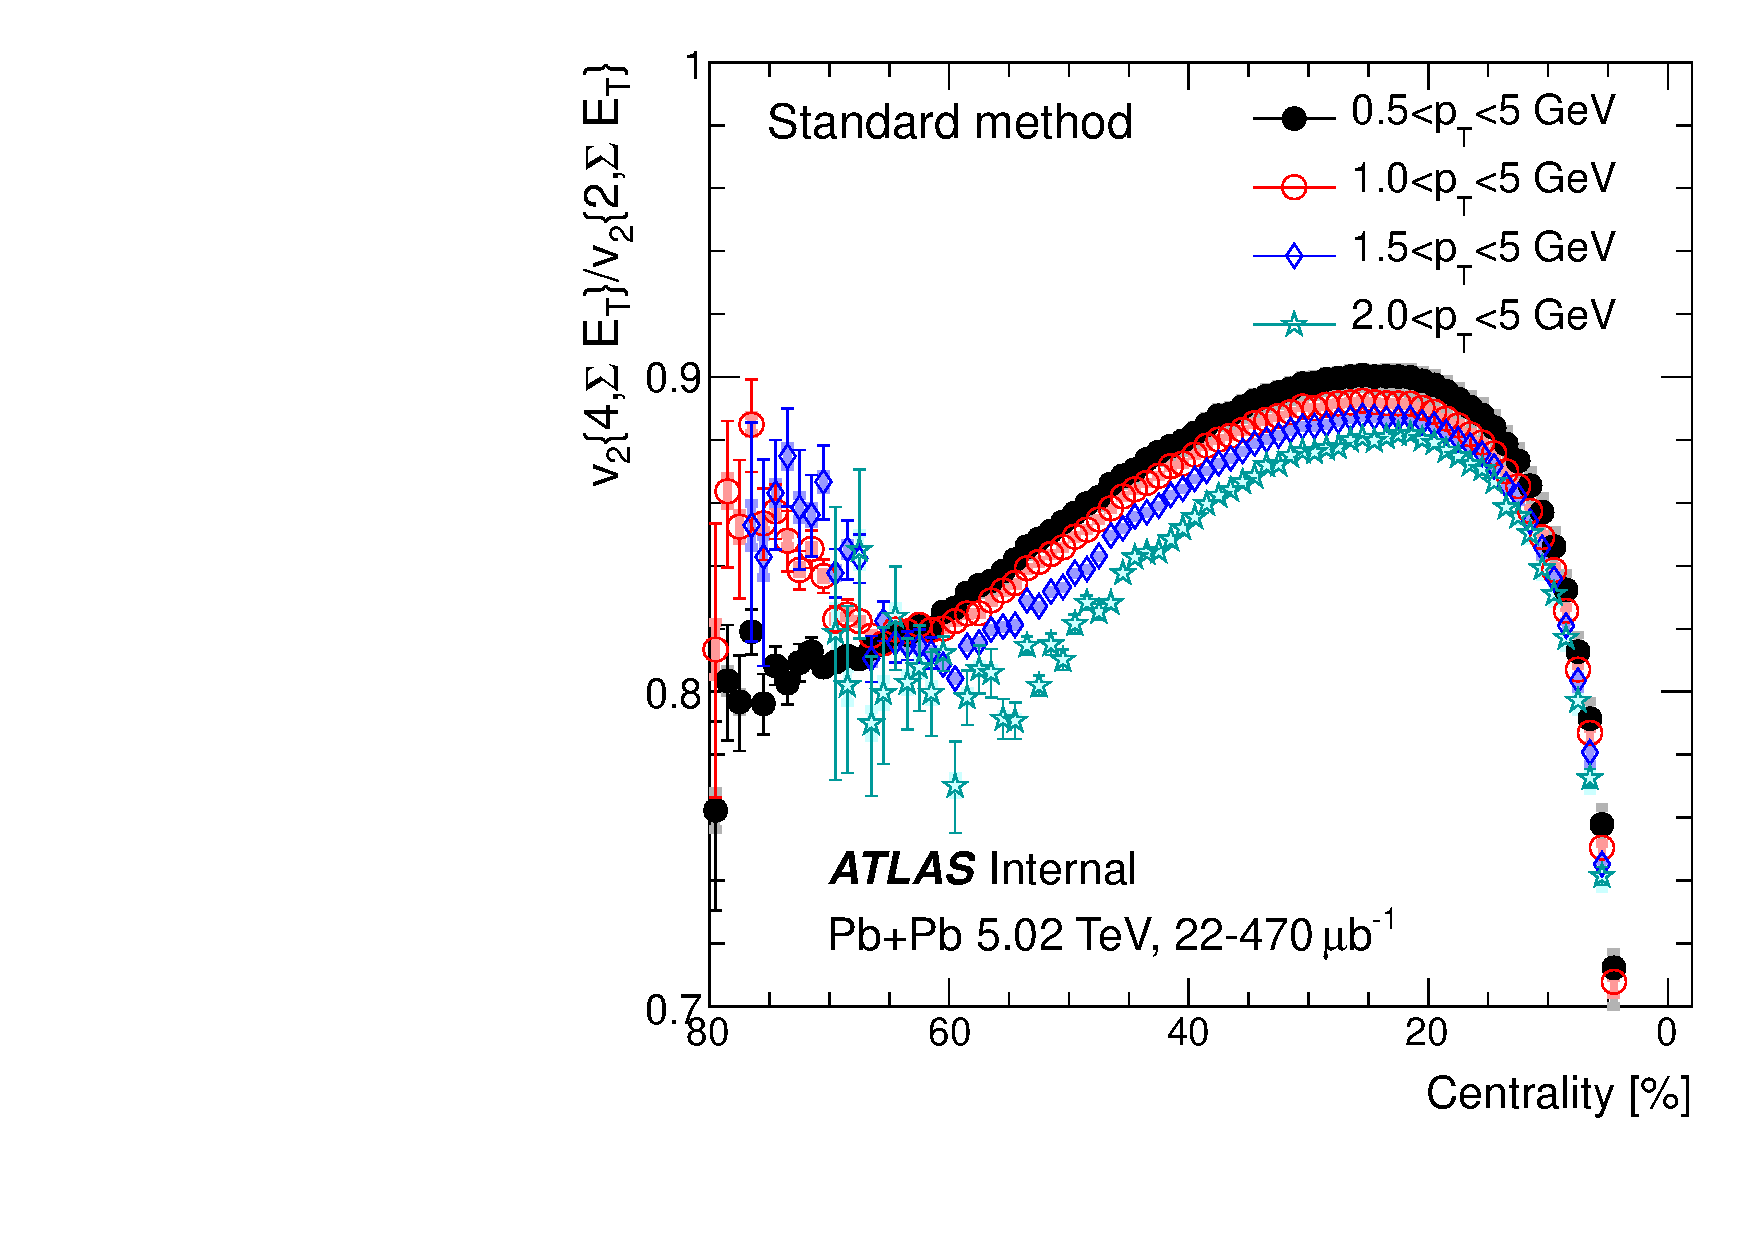
\includegraphics[width=.32\linewidth]{figs/sec_paper/comp_vn4vn2_har2_Cent.pdf}
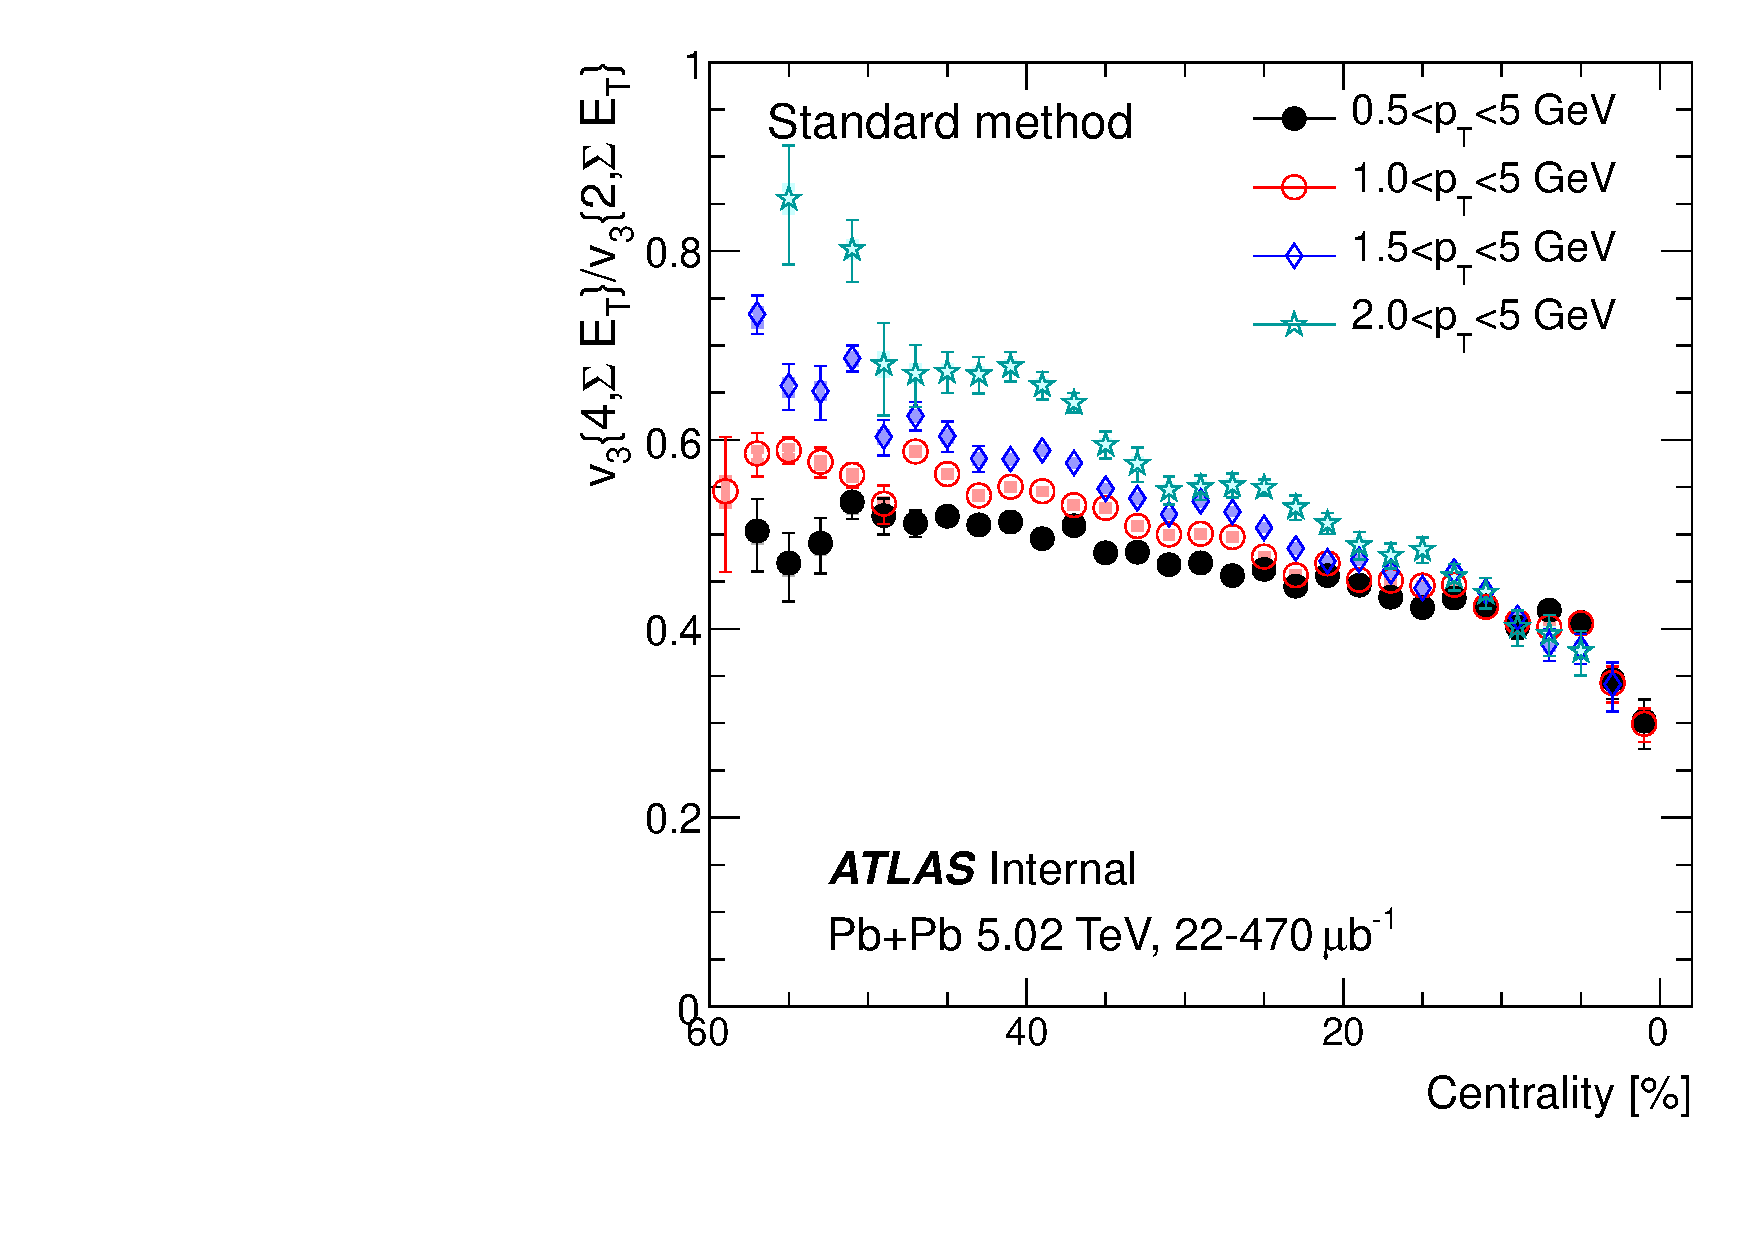
\includegraphics[width=.32\linewidth]{figs/sec_paper/comp_vn4vn2_har3_Cent.pdf}
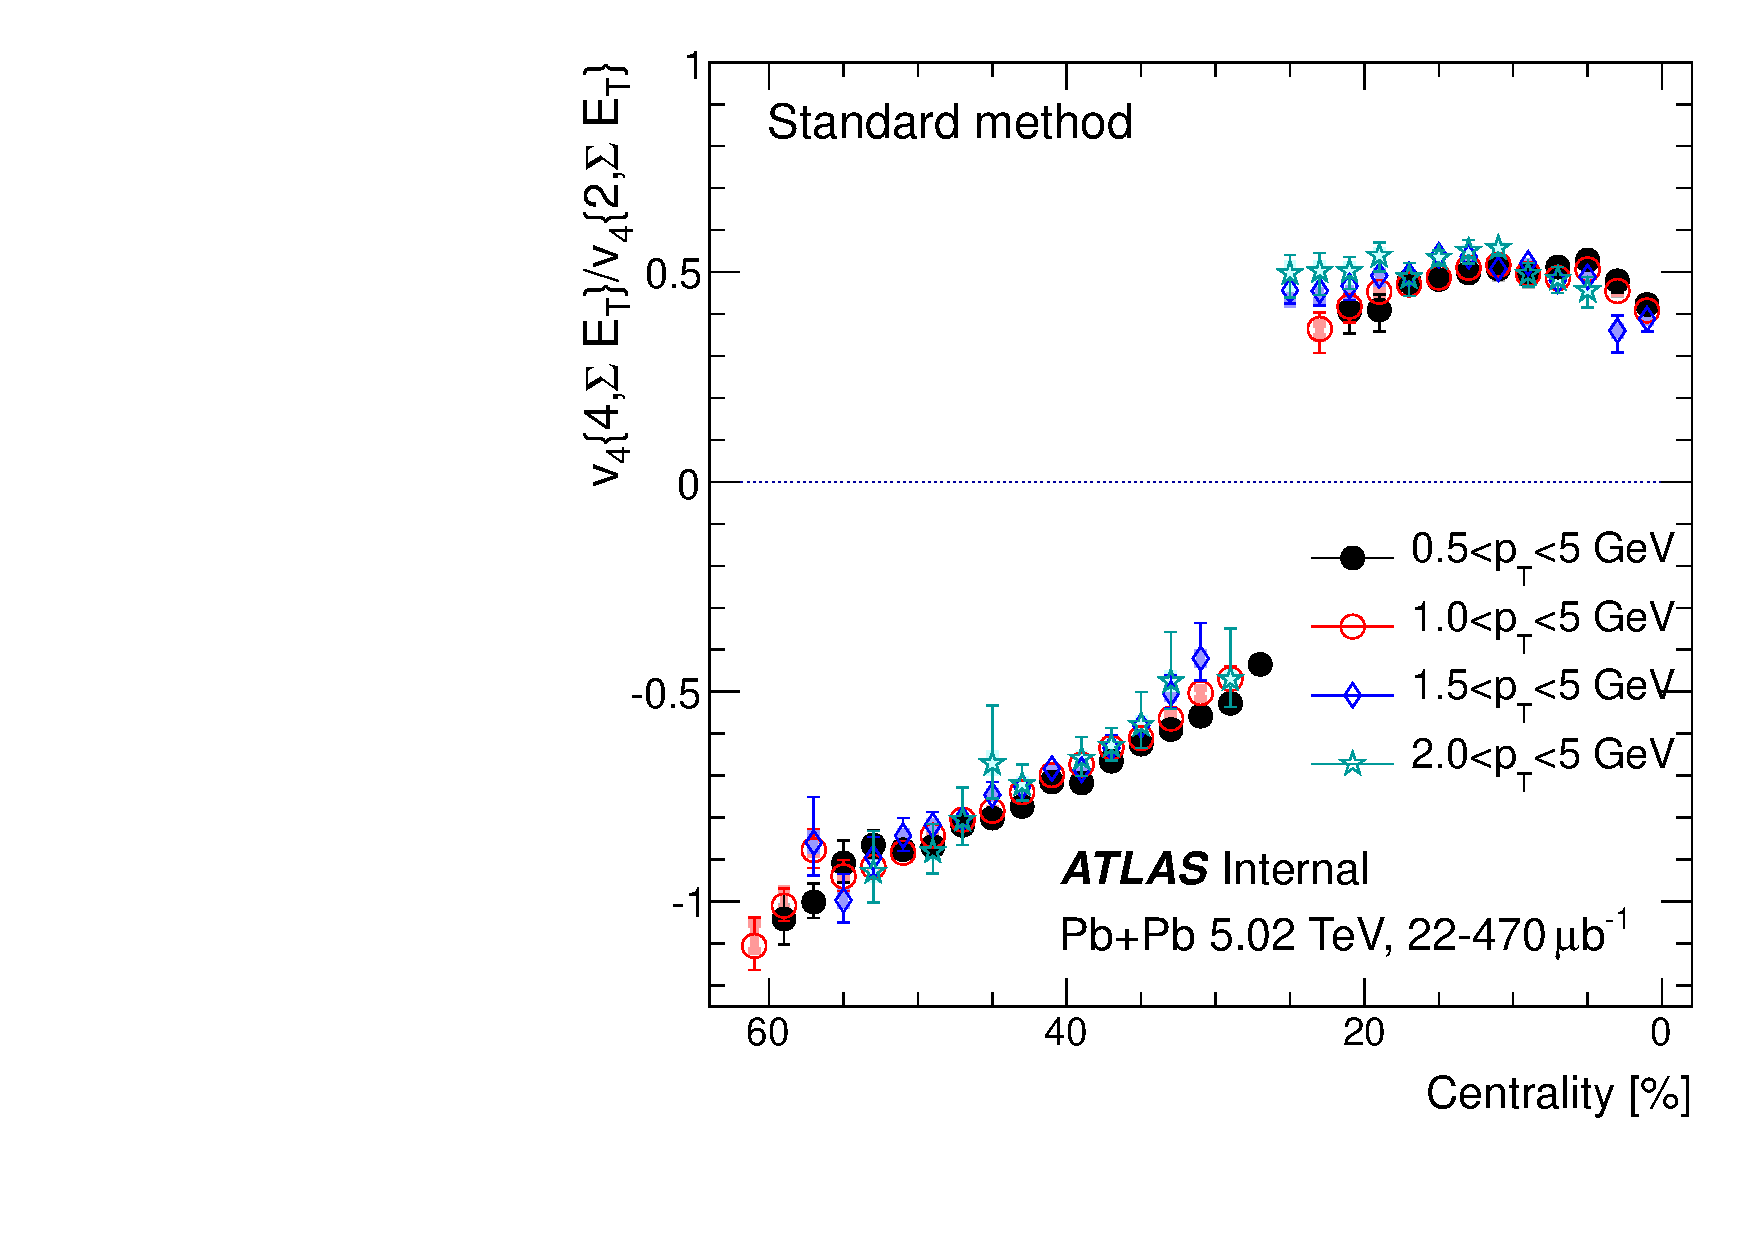
\includegraphics[width=.32\linewidth]{figs/sec_paper/comp_vn4vn2_har4_Cent.pdf}
\caption{Cumulant ratio $v_n\{4\}/v_n\{2\}$ as a function of centrality, calculated using standard method, with multiple $p_\text{T}$ ranges.}
\label{fig:paper_cr42}
\end{figure}

\subsection{Cumulant ratio $v_n\{6\}/v_n\{4\}$ with $n=2$ and comparison with CMS}

\begin{figure}[H]
\centering
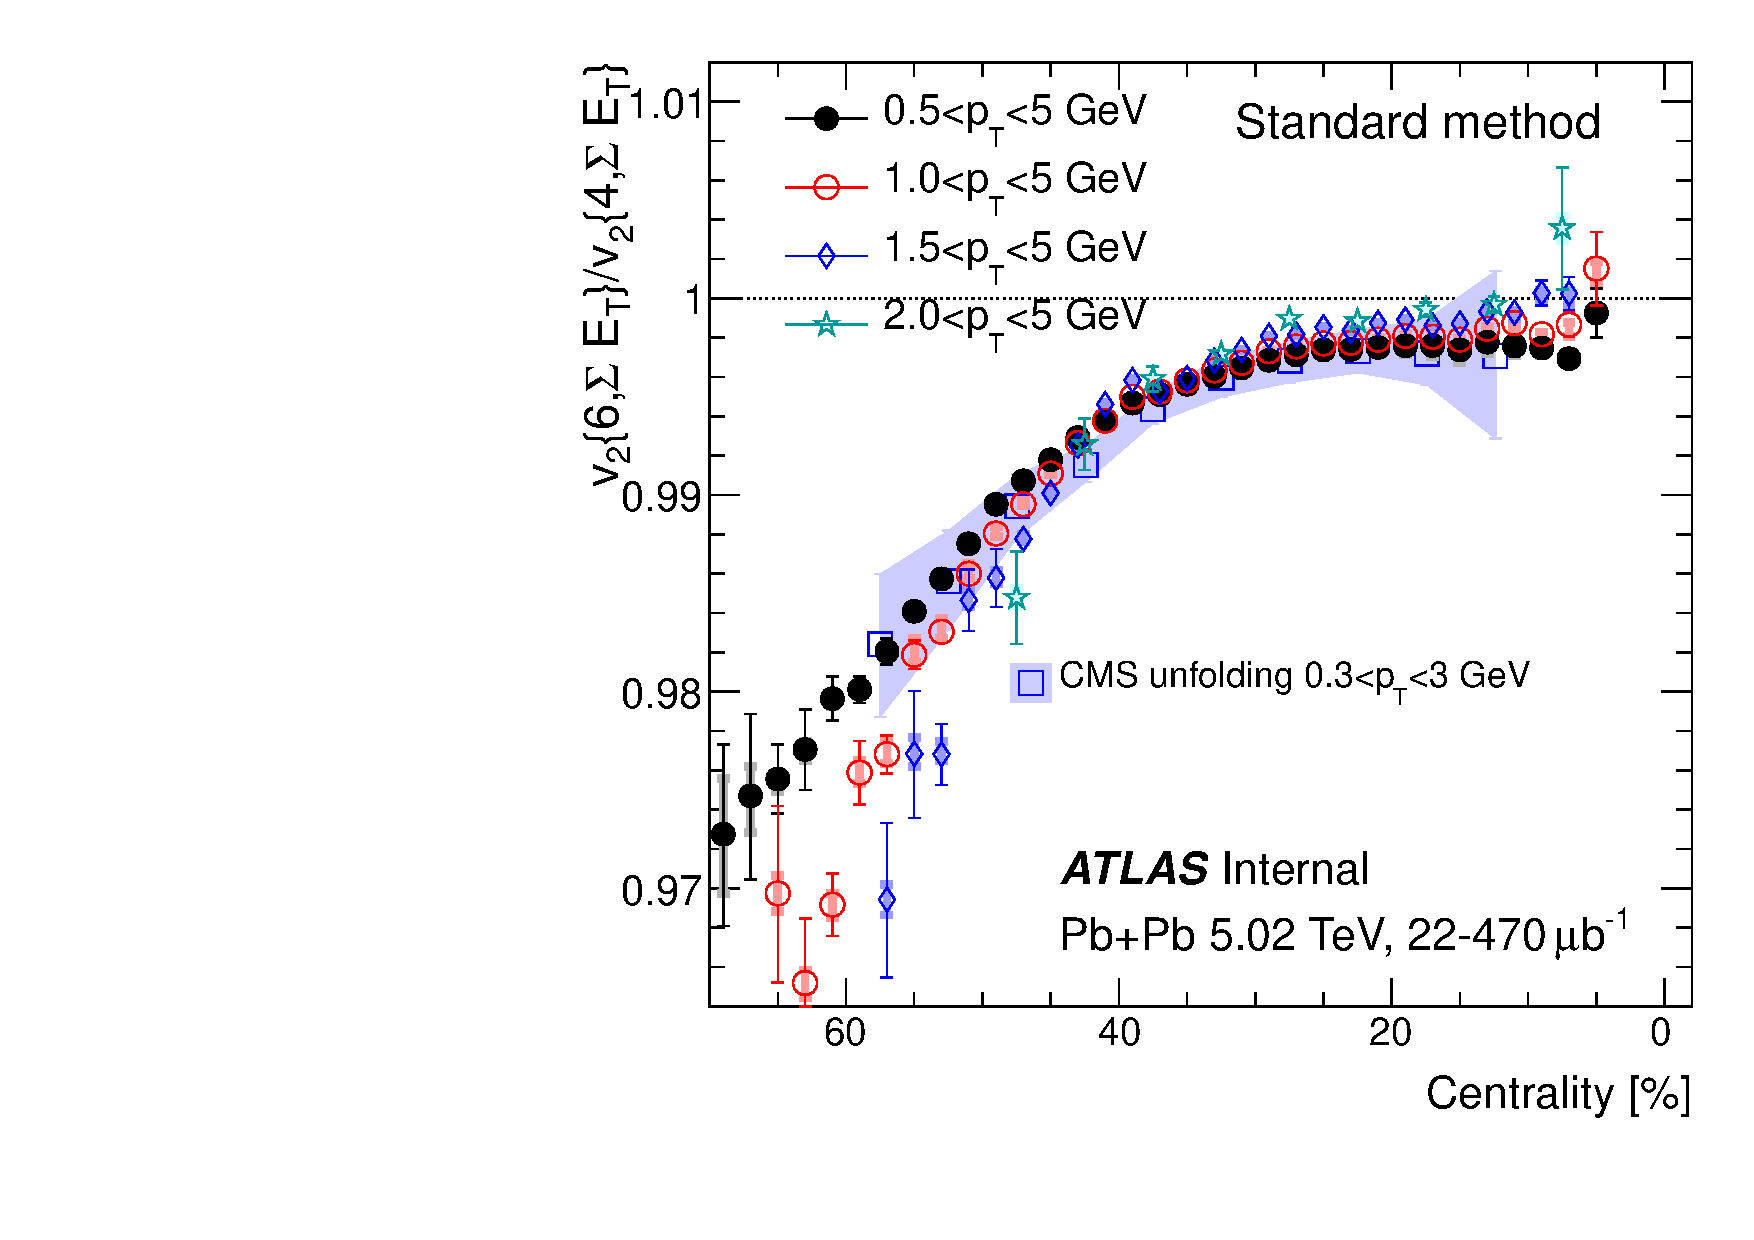
\includegraphics[width=.32\linewidth]{figs/sec_paper/comp_vn6vn4_har2_Cent.pdf}
\caption{Cumulant ratio $v_n\{6\}/v_n\{4\}$ as a function of centrality, calculated using standard method, with multiple $p_\text{T}$ ranges.}
\label{fig:paper_cr64}
\end{figure}

\subsection{Symmetric and asymmetric cumulant}

\begin{figure}[H]
\centering
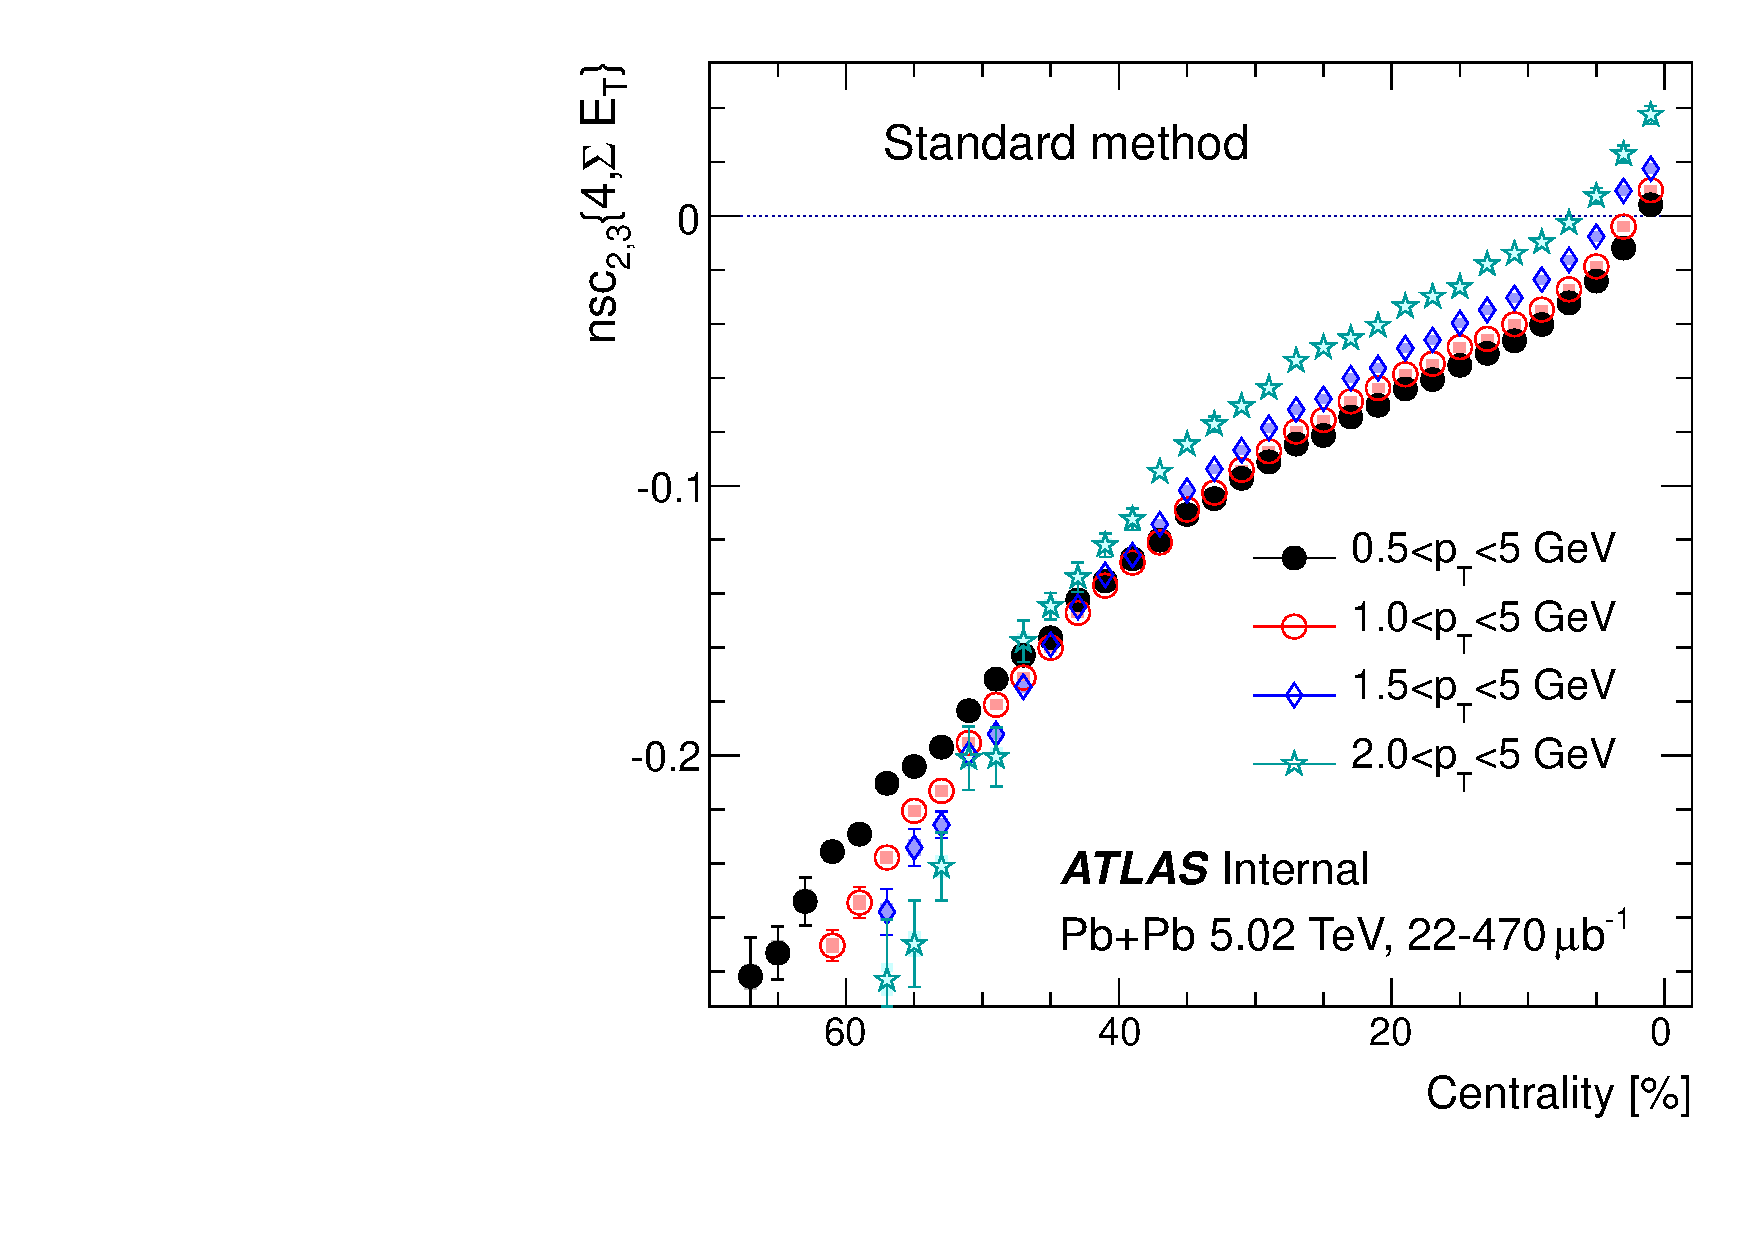
\includegraphics[width=.32\linewidth]{figs/sec_paper/comp_nsc_har2_Cent.pdf}
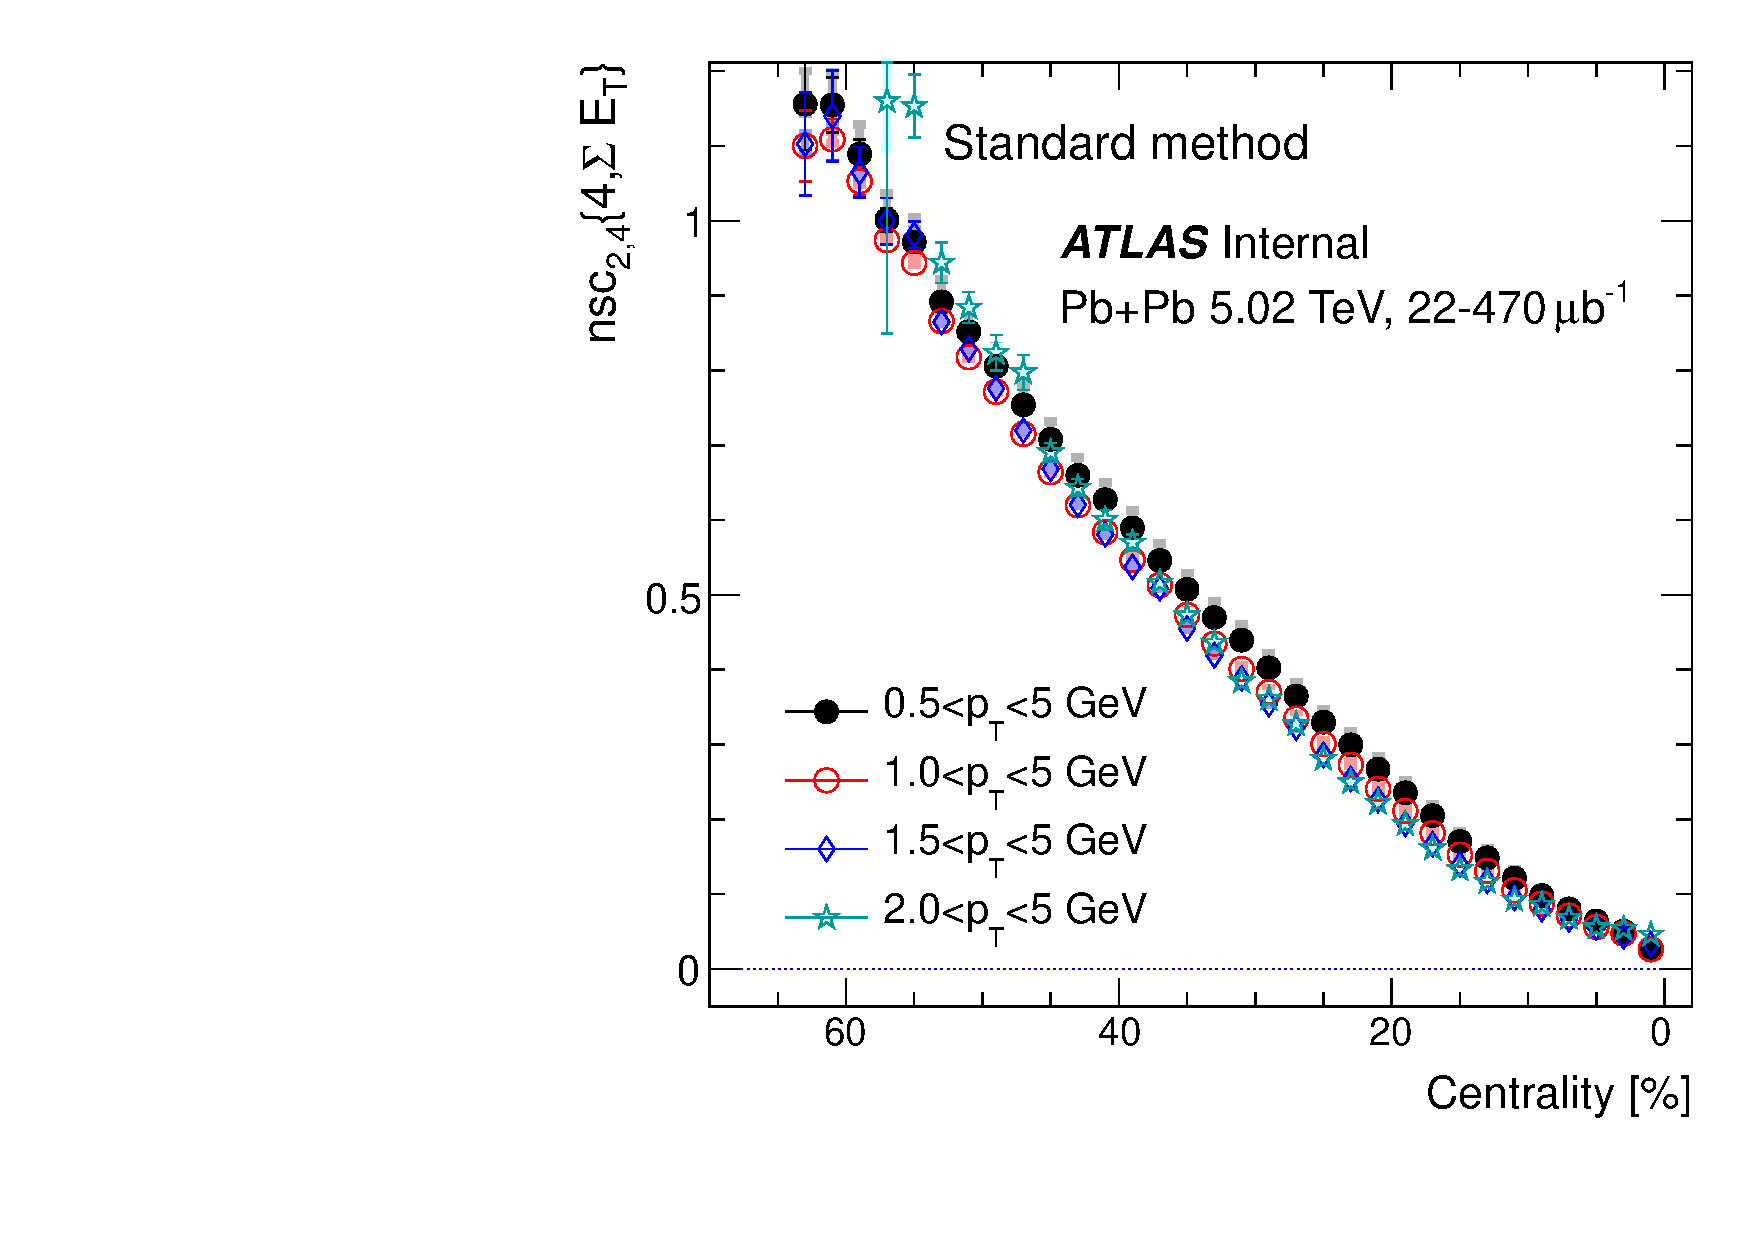
\includegraphics[width=.32\linewidth]{figs/sec_paper/comp_nsc_har3_Cent.pdf}
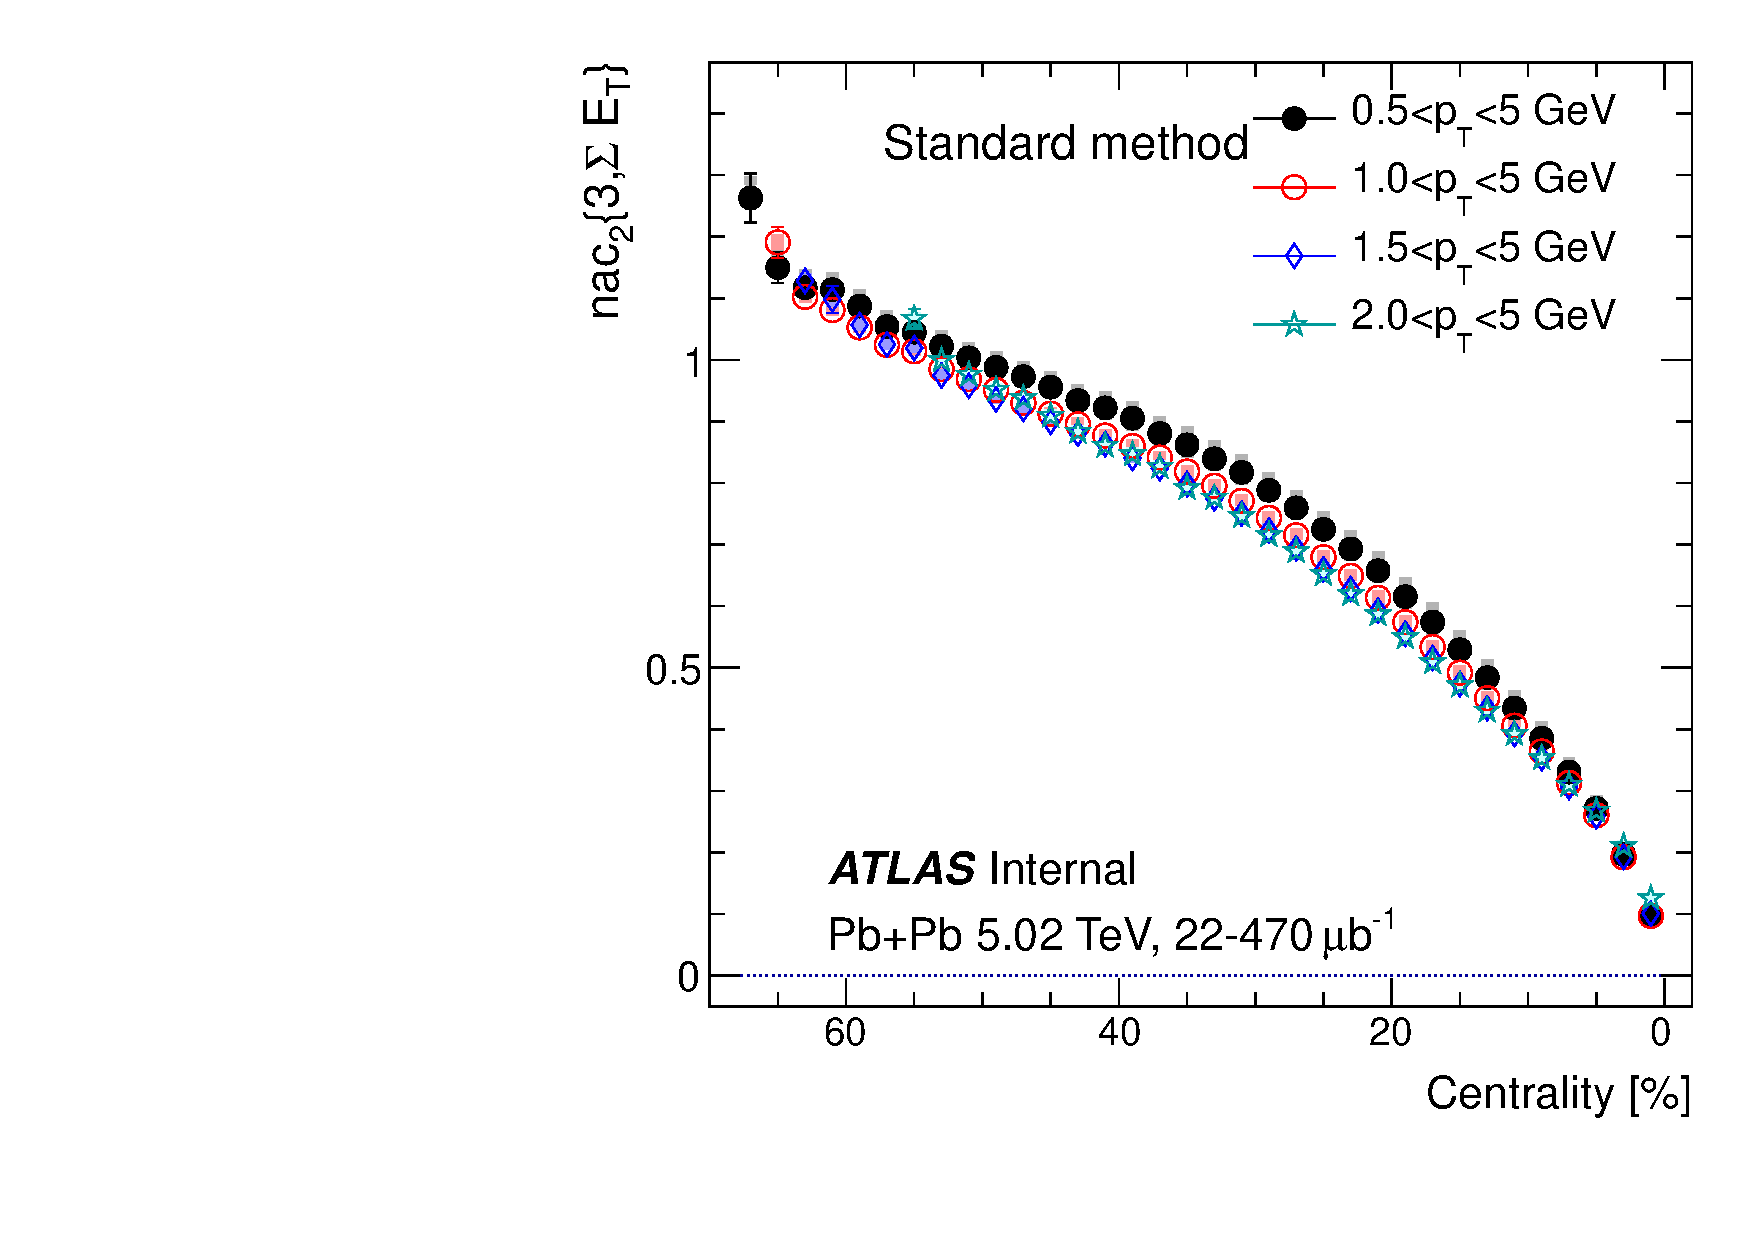
\includegraphics[width=.32\linewidth]{figs/sec_paper/comp_nac_har2_Cent.pdf}
\caption{Normalized symmetric and asymmetric cumulants as a function of centrality, calculated using standard method, with multiple $p_\text{T}$ ranges.}
\label{fig:paper_nsc}
\end{figure}

\begin{figure}[H]
\centering
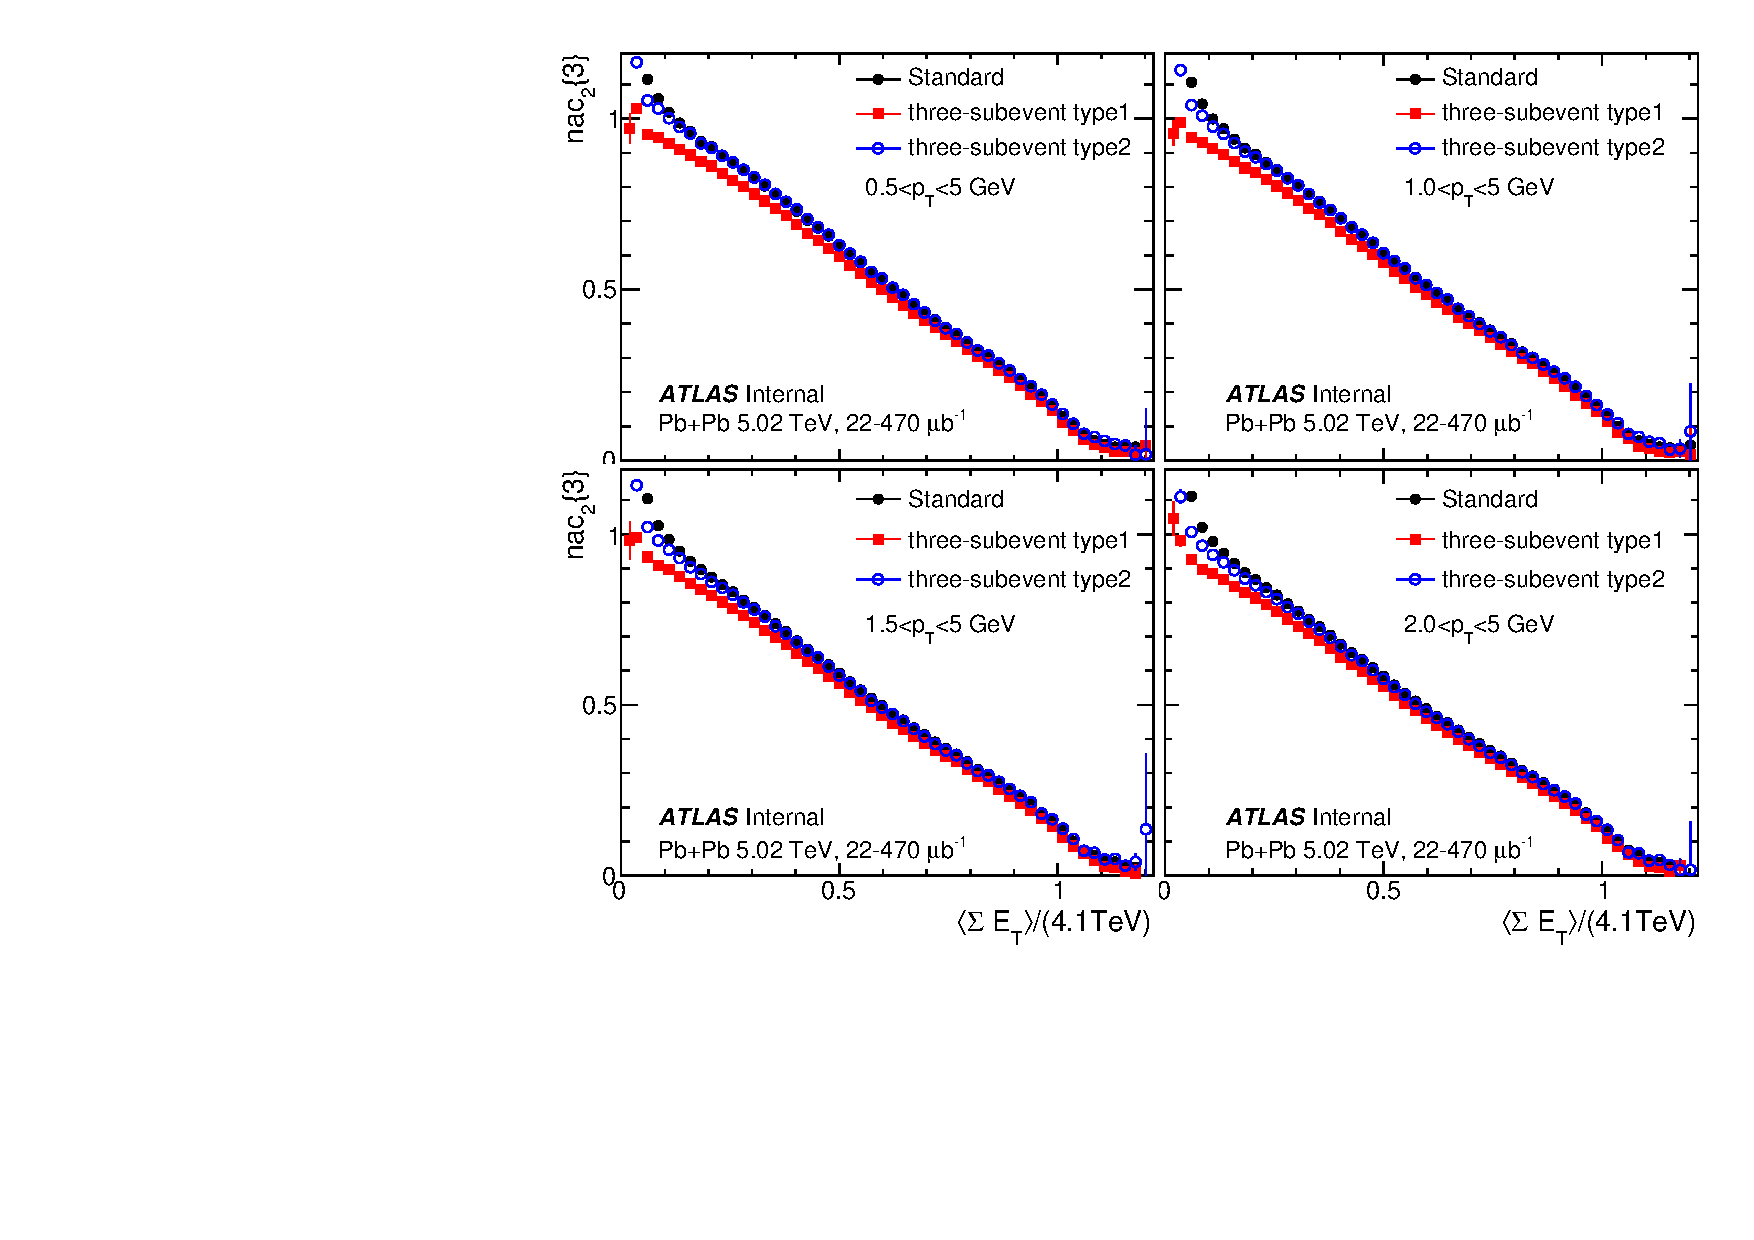
\includegraphics[width=.6\linewidth]{figs/sec_paper/nac_decorr1.pdf}
\caption{The $nac_2\{3\}$ from the standard method (solid circles),three-subevent method with $V_4$ defined in subevent a or c (solid squares) and three-subevent method with $V_4$ defined in subevent b (open circles). Different panels correspond to different $p_\text{T}$ ranges. Only statistical uncertainties are shown.}
\label{fig:paper_nac_decorr1}
\end{figure}

\begin{figure}[H]
\centering
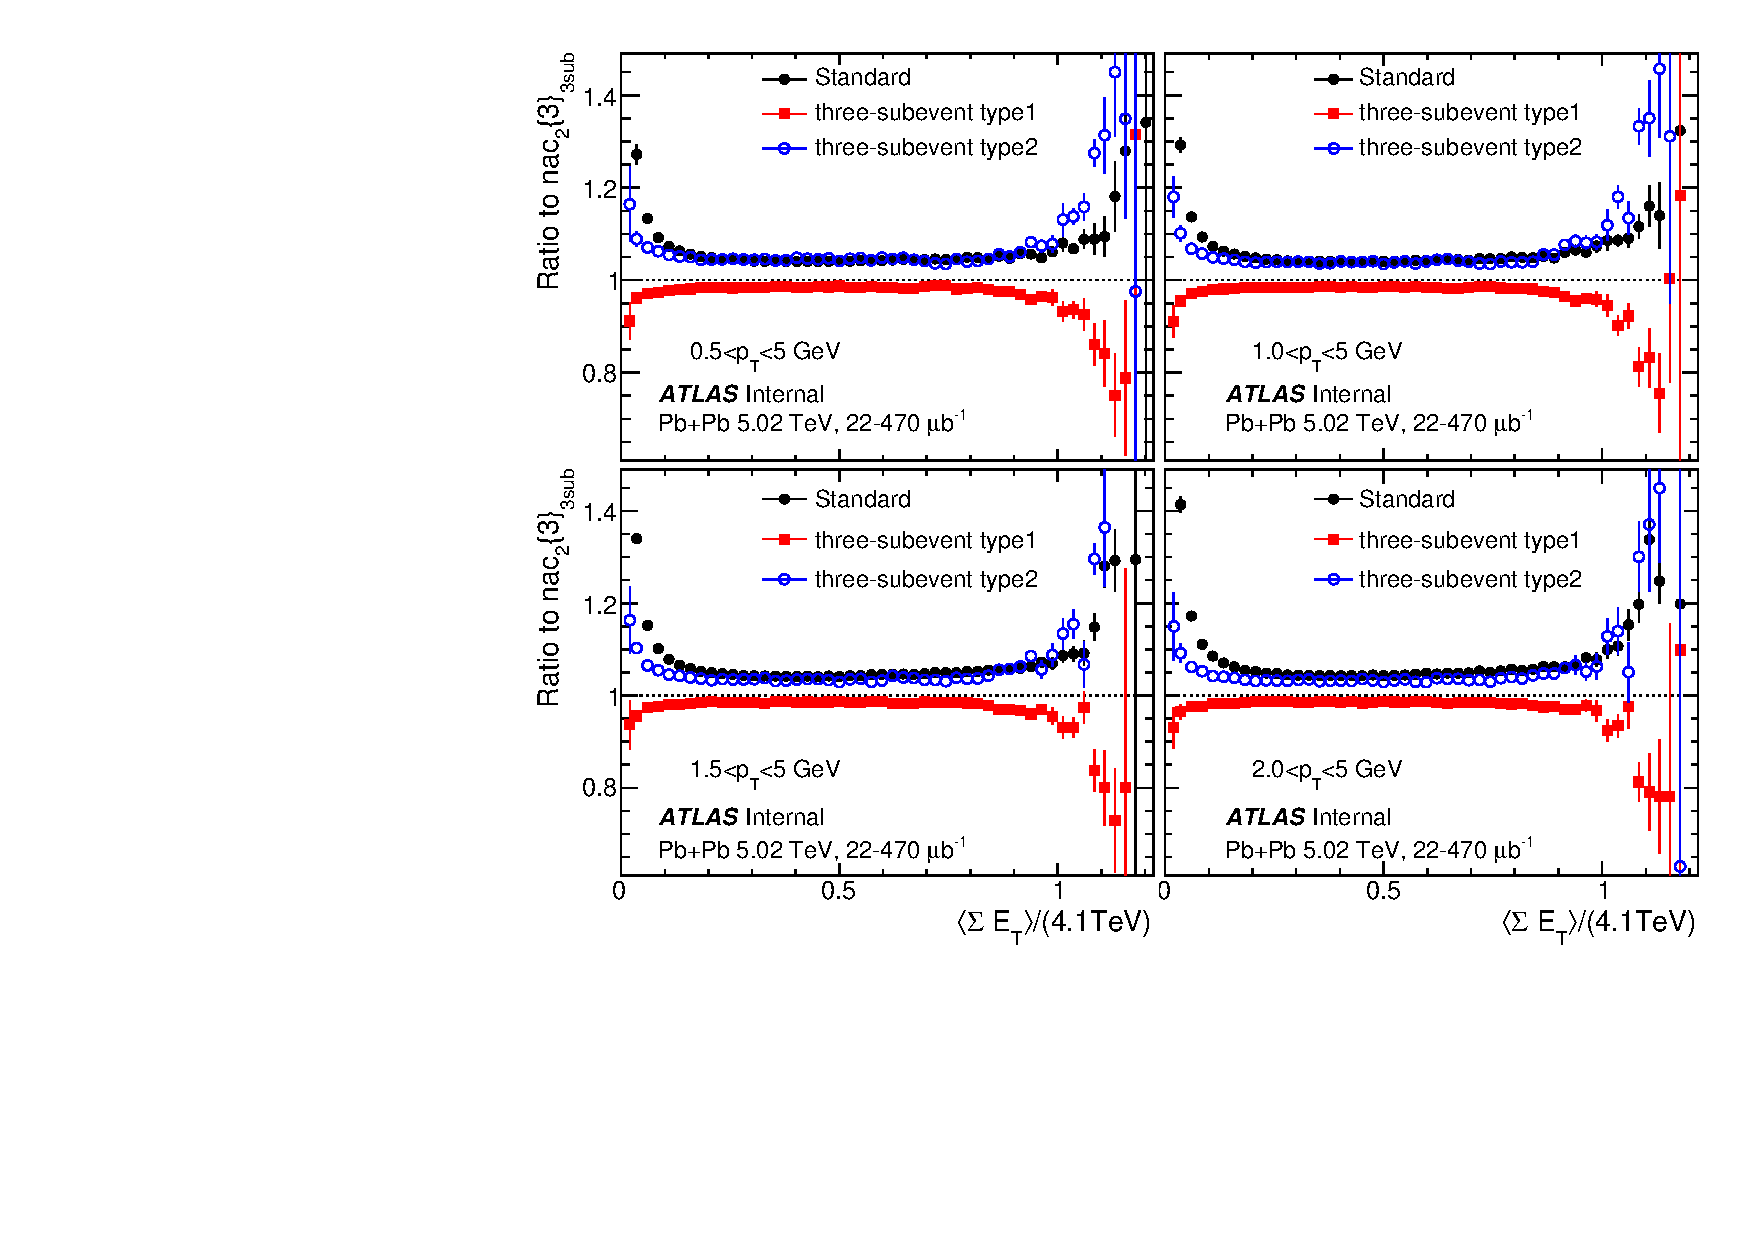
\includegraphics[width=.6\linewidth]{figs/sec_paper/nac_decorr2.pdf}
\caption{The ratio of $nac_2\{3\}$ from the standard method (solid circles), three-subevent method with $V_4$ defined in subevent a or c (solid squares) and three-subevent method with $V_4$ defined in subevent b (open circles) to $nac_2\{3\}$ from the three-subevent method combined. Different panels correspond to different $p_\text{T}$ ranges. Only statistical uncertainties are shown.}
\label{fig:paper_nac_decorr2}
\end{figure}

\subsection{Volume fluctuation}

\begin{figure}[H]
\centering
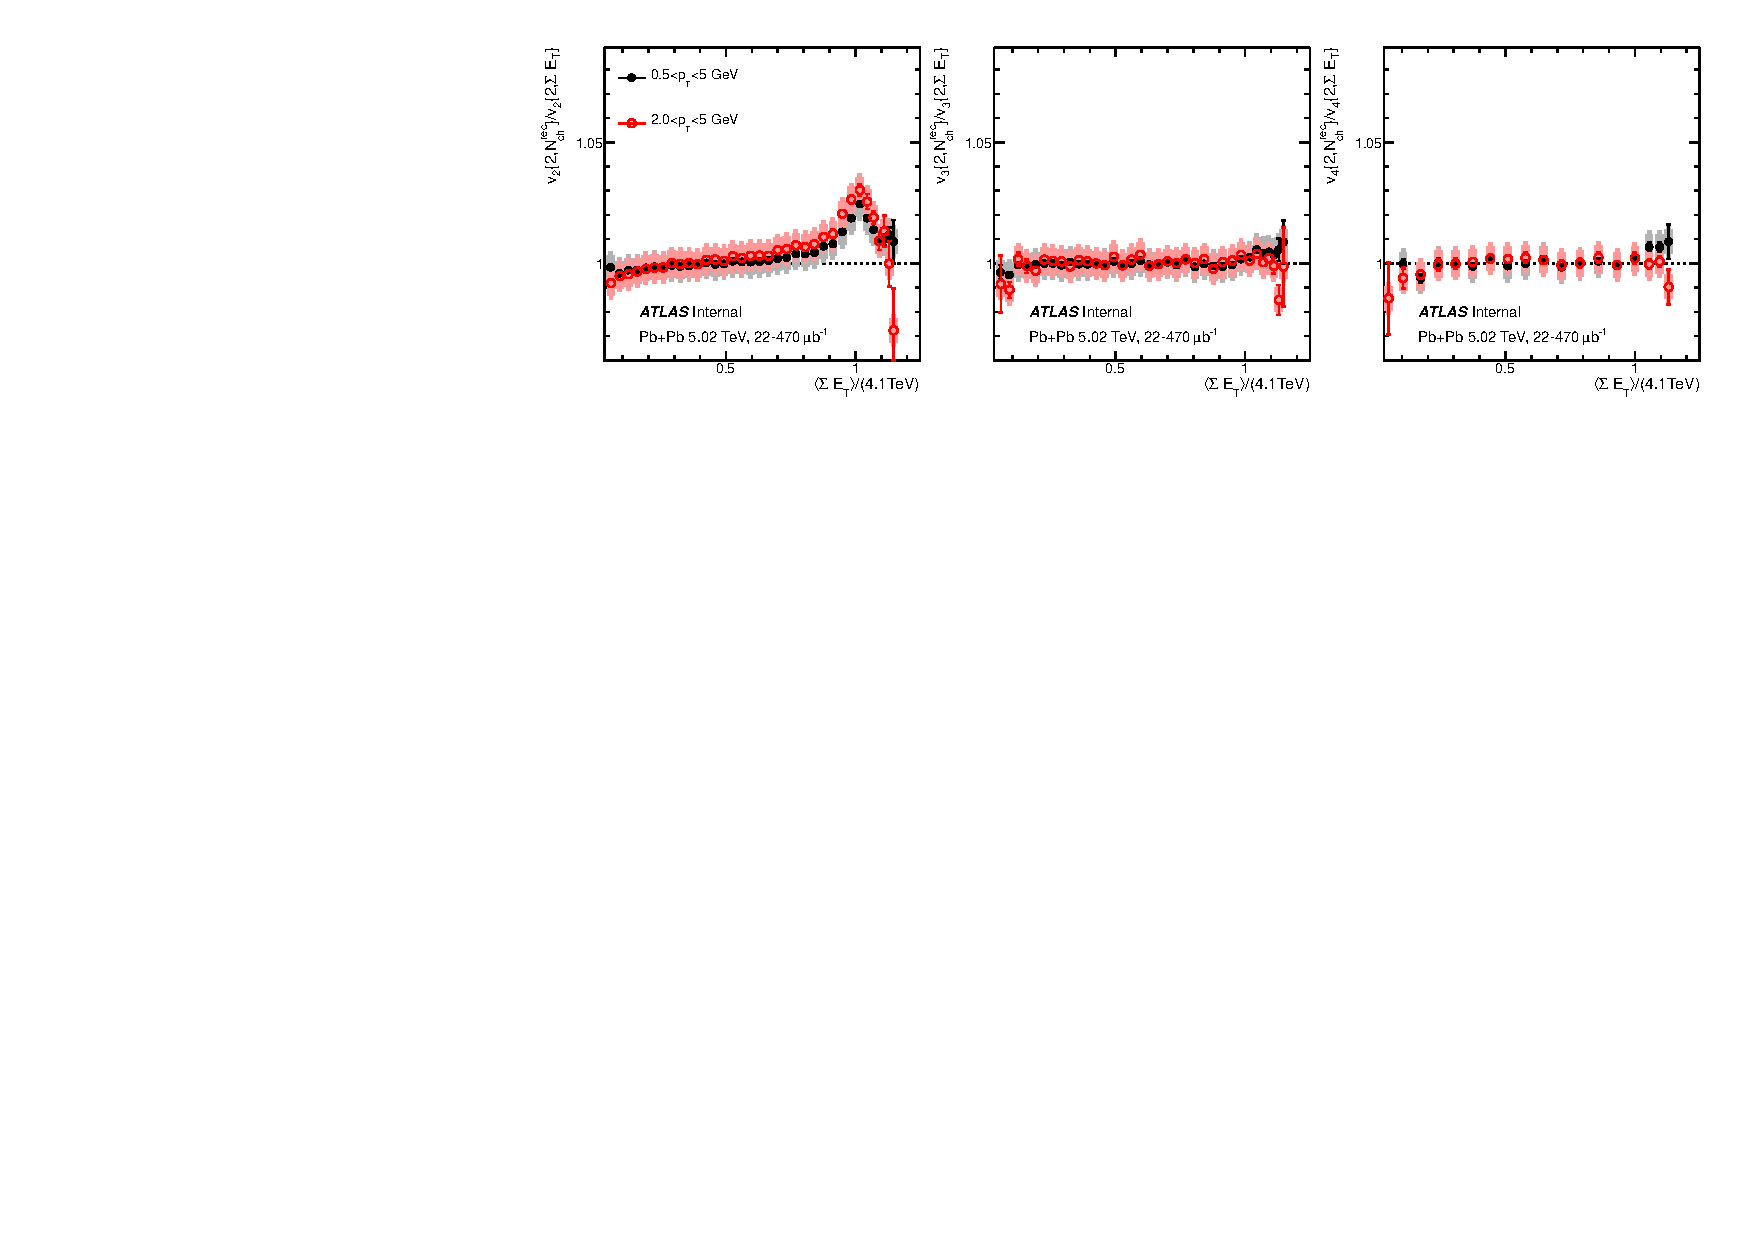
\includegraphics[width=.96\linewidth]{figs/sec_paper/comp_vn2rat_FCal.pdf}
\caption{Check of volume fluctuation for 2-particle flow cumulant.}
\label{fig:paper_vf_v2}
\end{figure}

\begin{figure}[H]
\centering
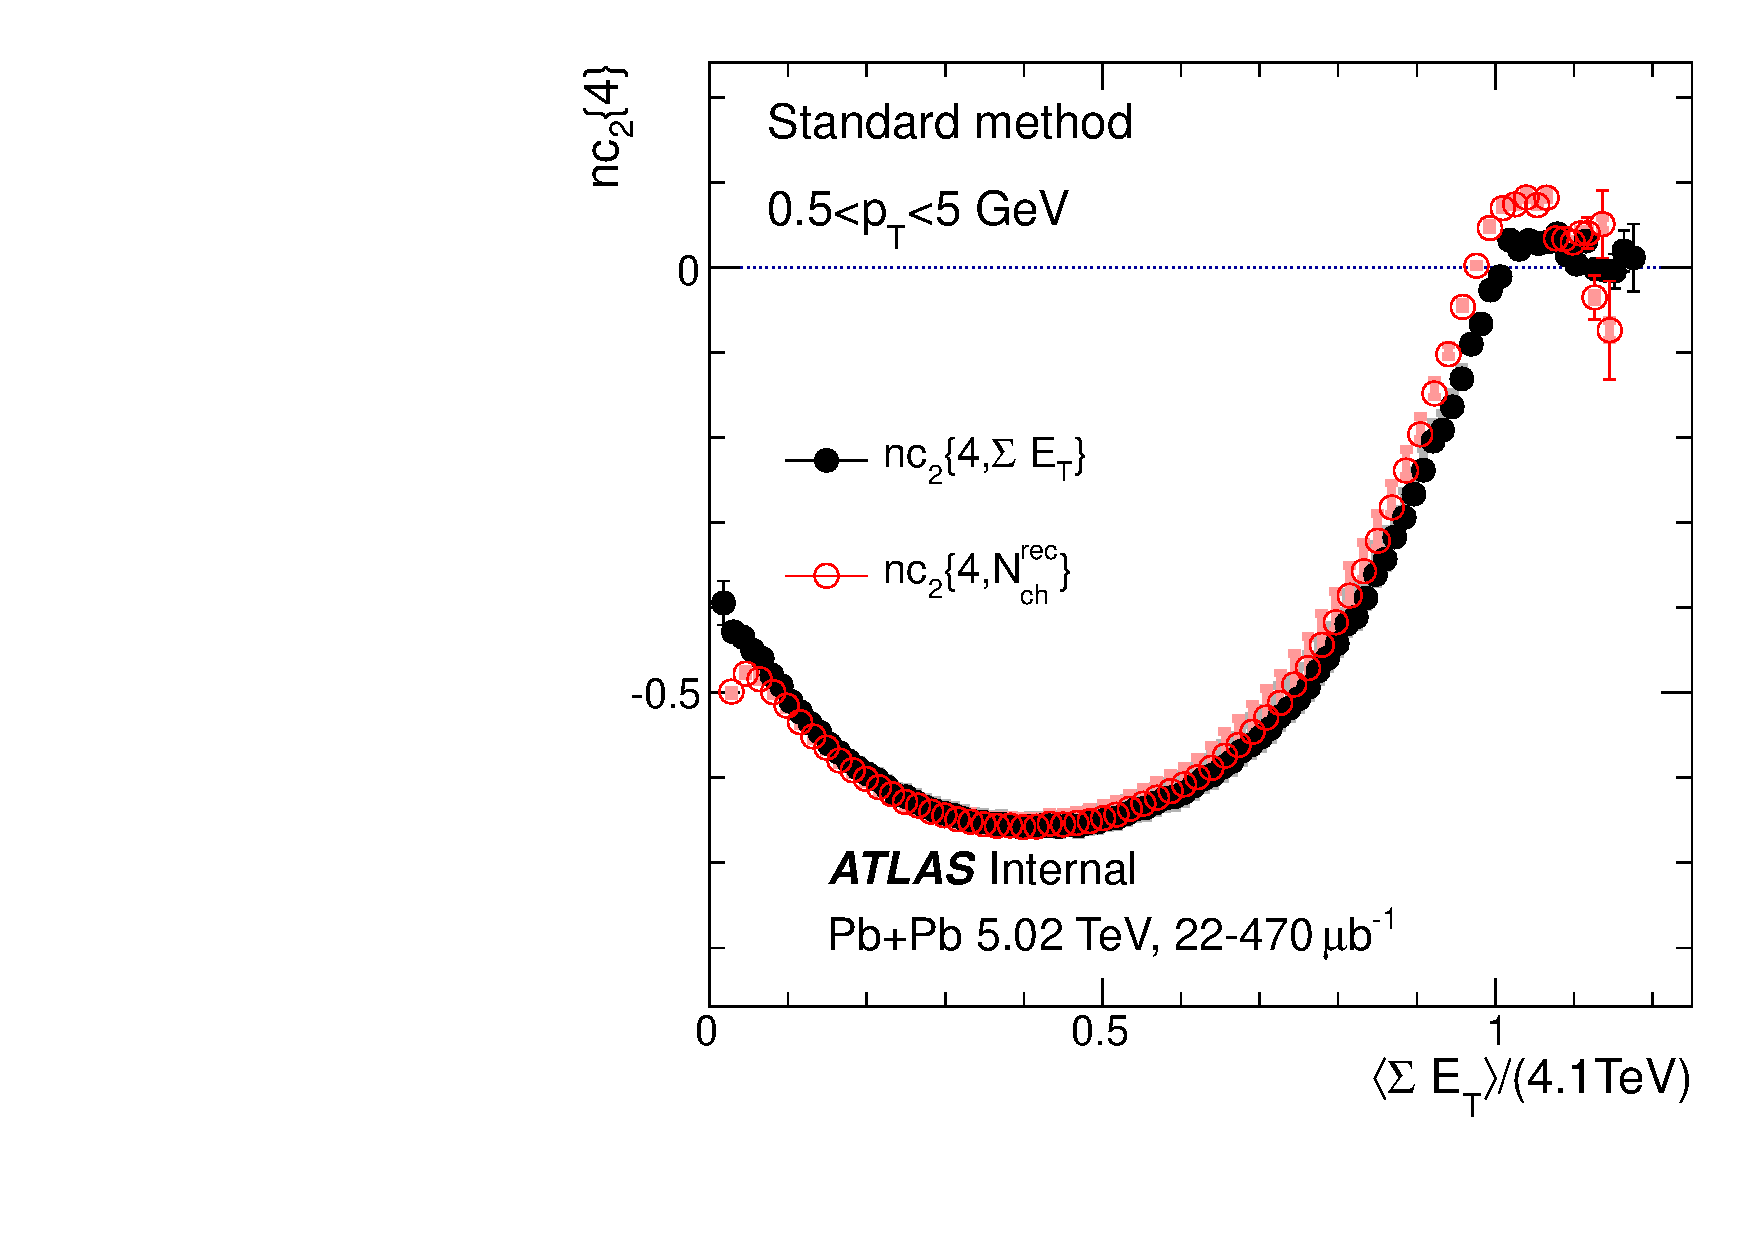
\includegraphics[width=.32\linewidth]{figs/sec_paper/comp_nc4comp_t0_har2_pt0.pdf}
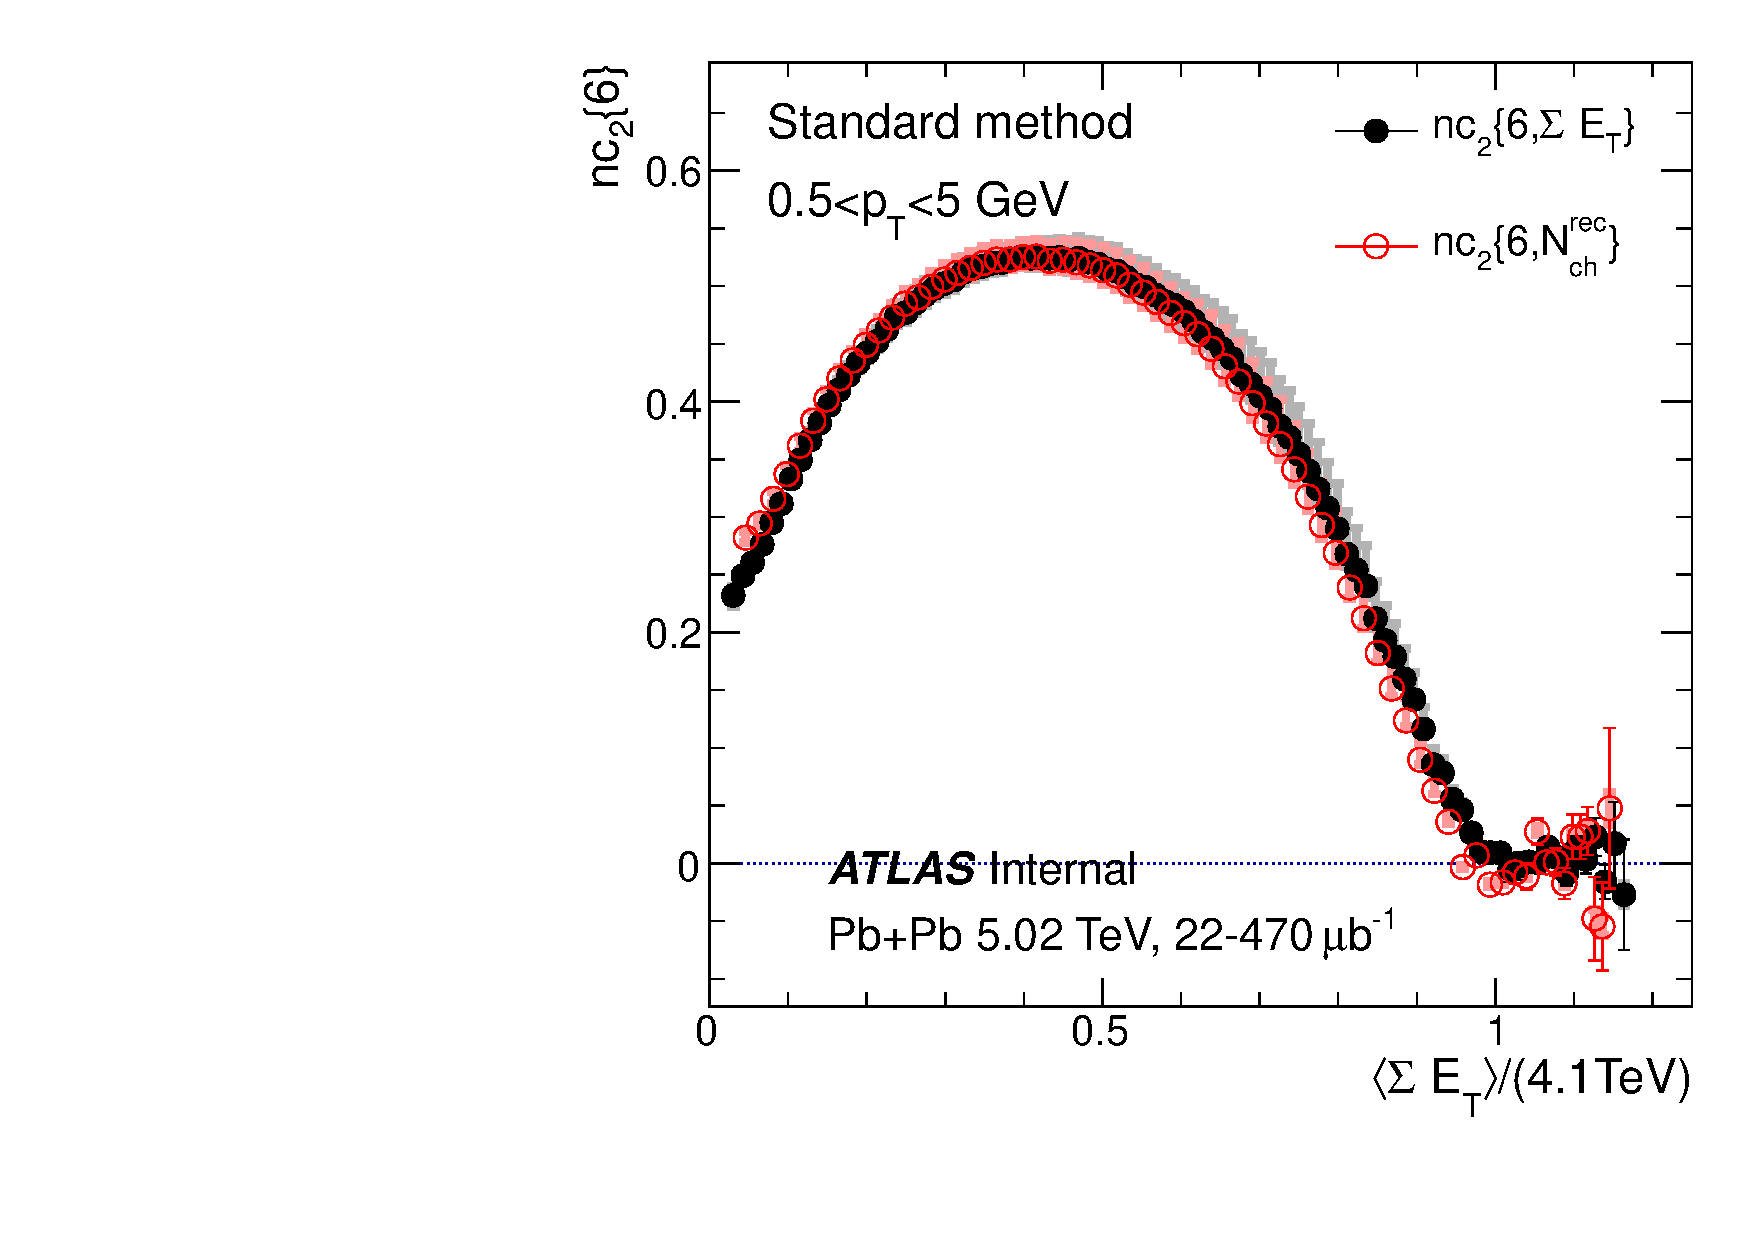
\includegraphics[width=.32\linewidth]{figs/sec_paper/comp_nc6comp_t0_har2_pt0.pdf}
\caption{Check of volume fluctuation for 4- and 6-particle flow cumulant.}
\label{fig:paper_vf_v4}
\end{figure}

\begin{figure}[H]
\centering
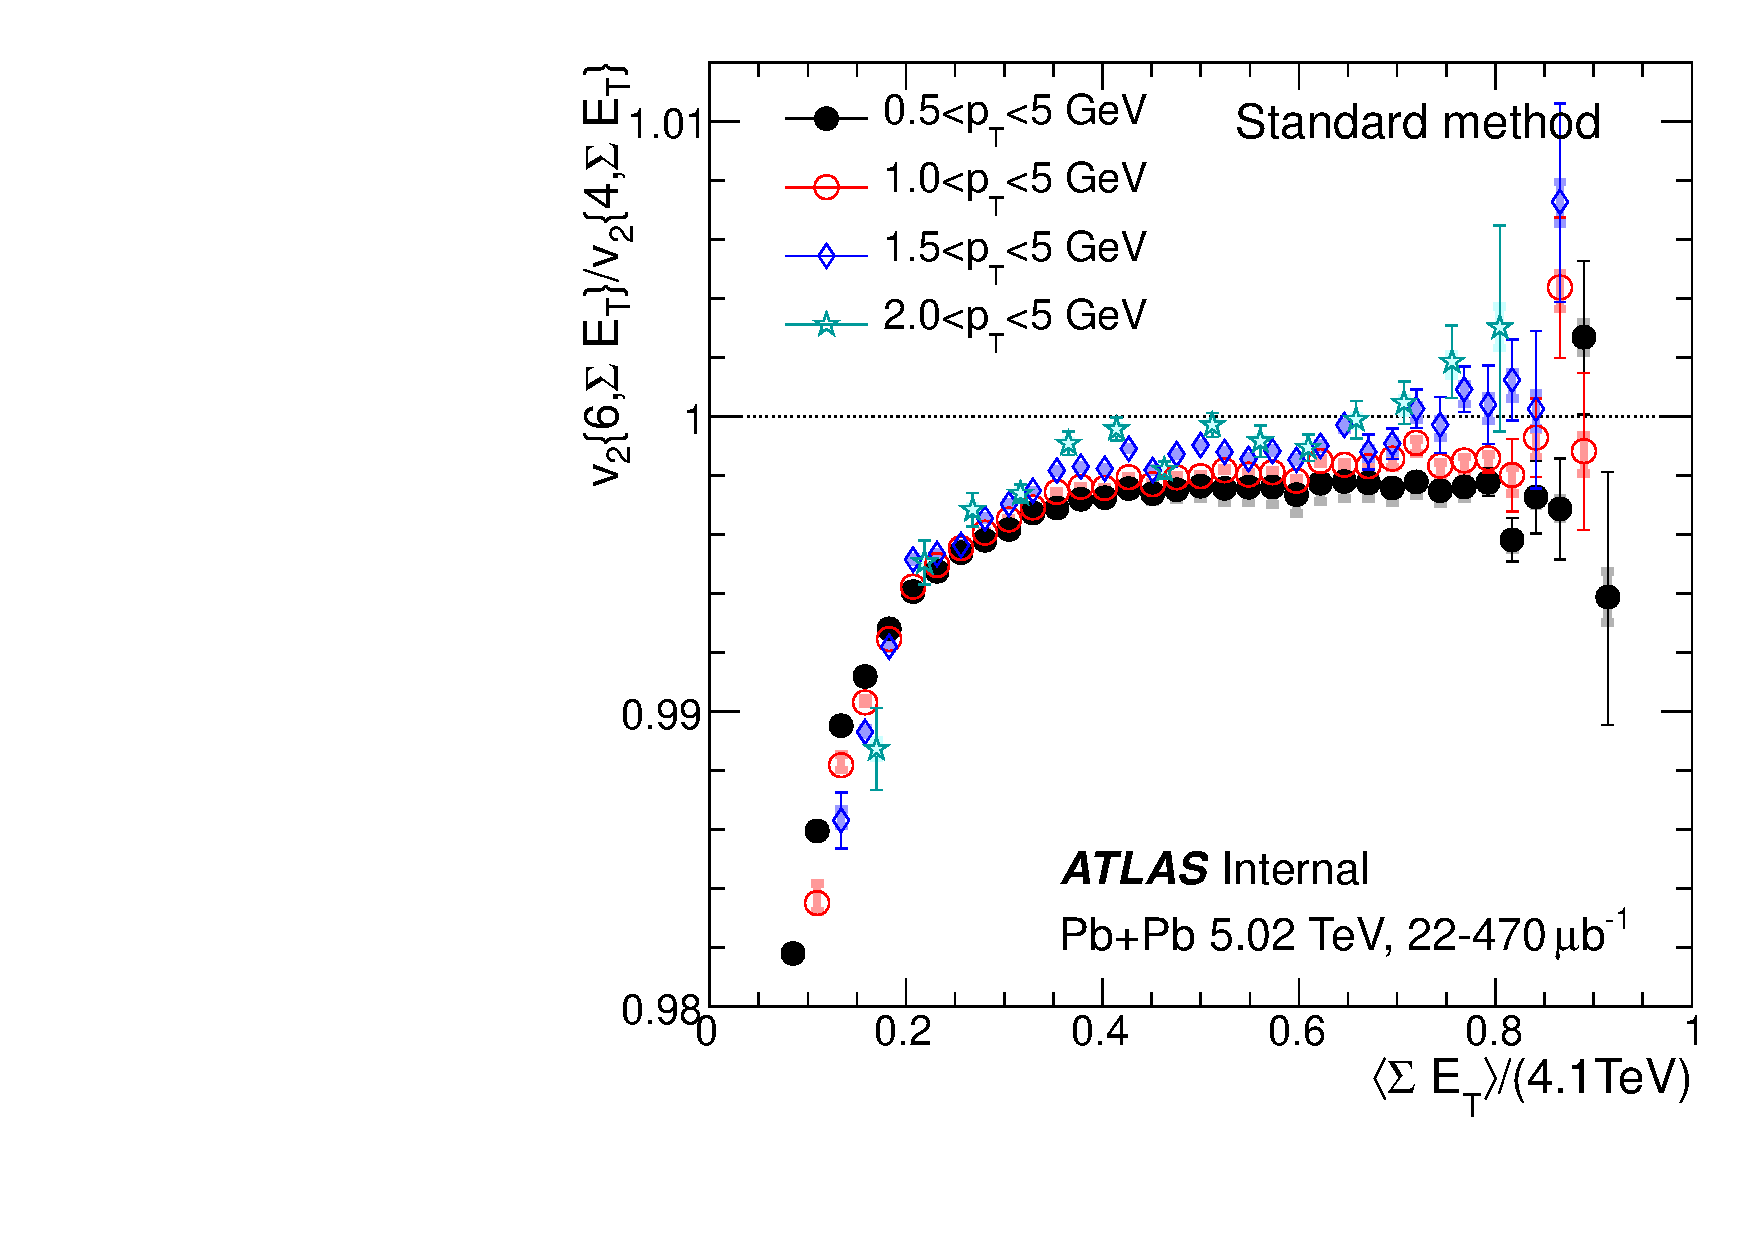
\includegraphics[width=.32\linewidth]{figs/sec_paper/comp_vn6vn4_har2_FCal.pdf}
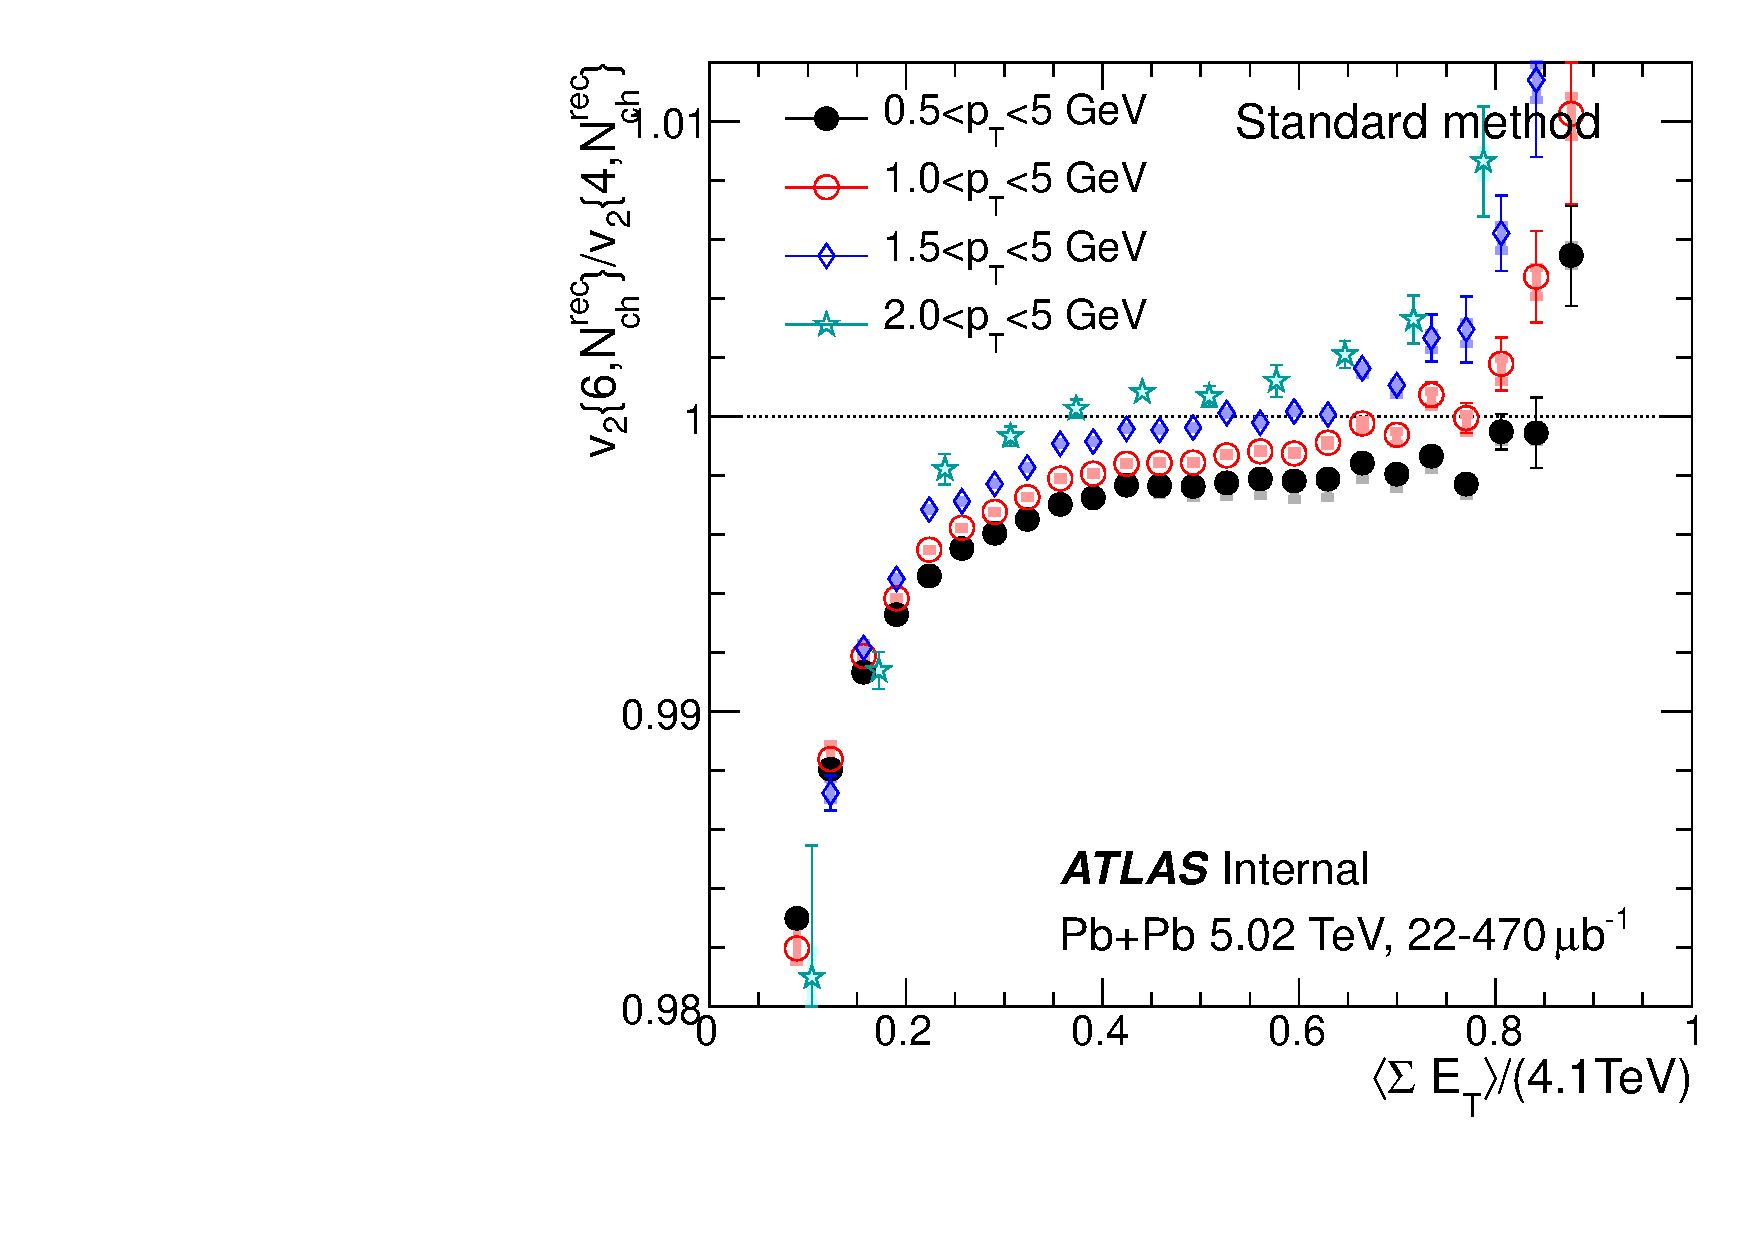
\includegraphics[width=.32\linewidth]{figs/sec_paper/comp_vn6vn4_har2_Nchb.pdf}
\caption{Check of volume fluctuation for cumulant ratios.}
\label{fig:paper_vf_cr}
\end{figure}

\begin{figure}[H]
\centering
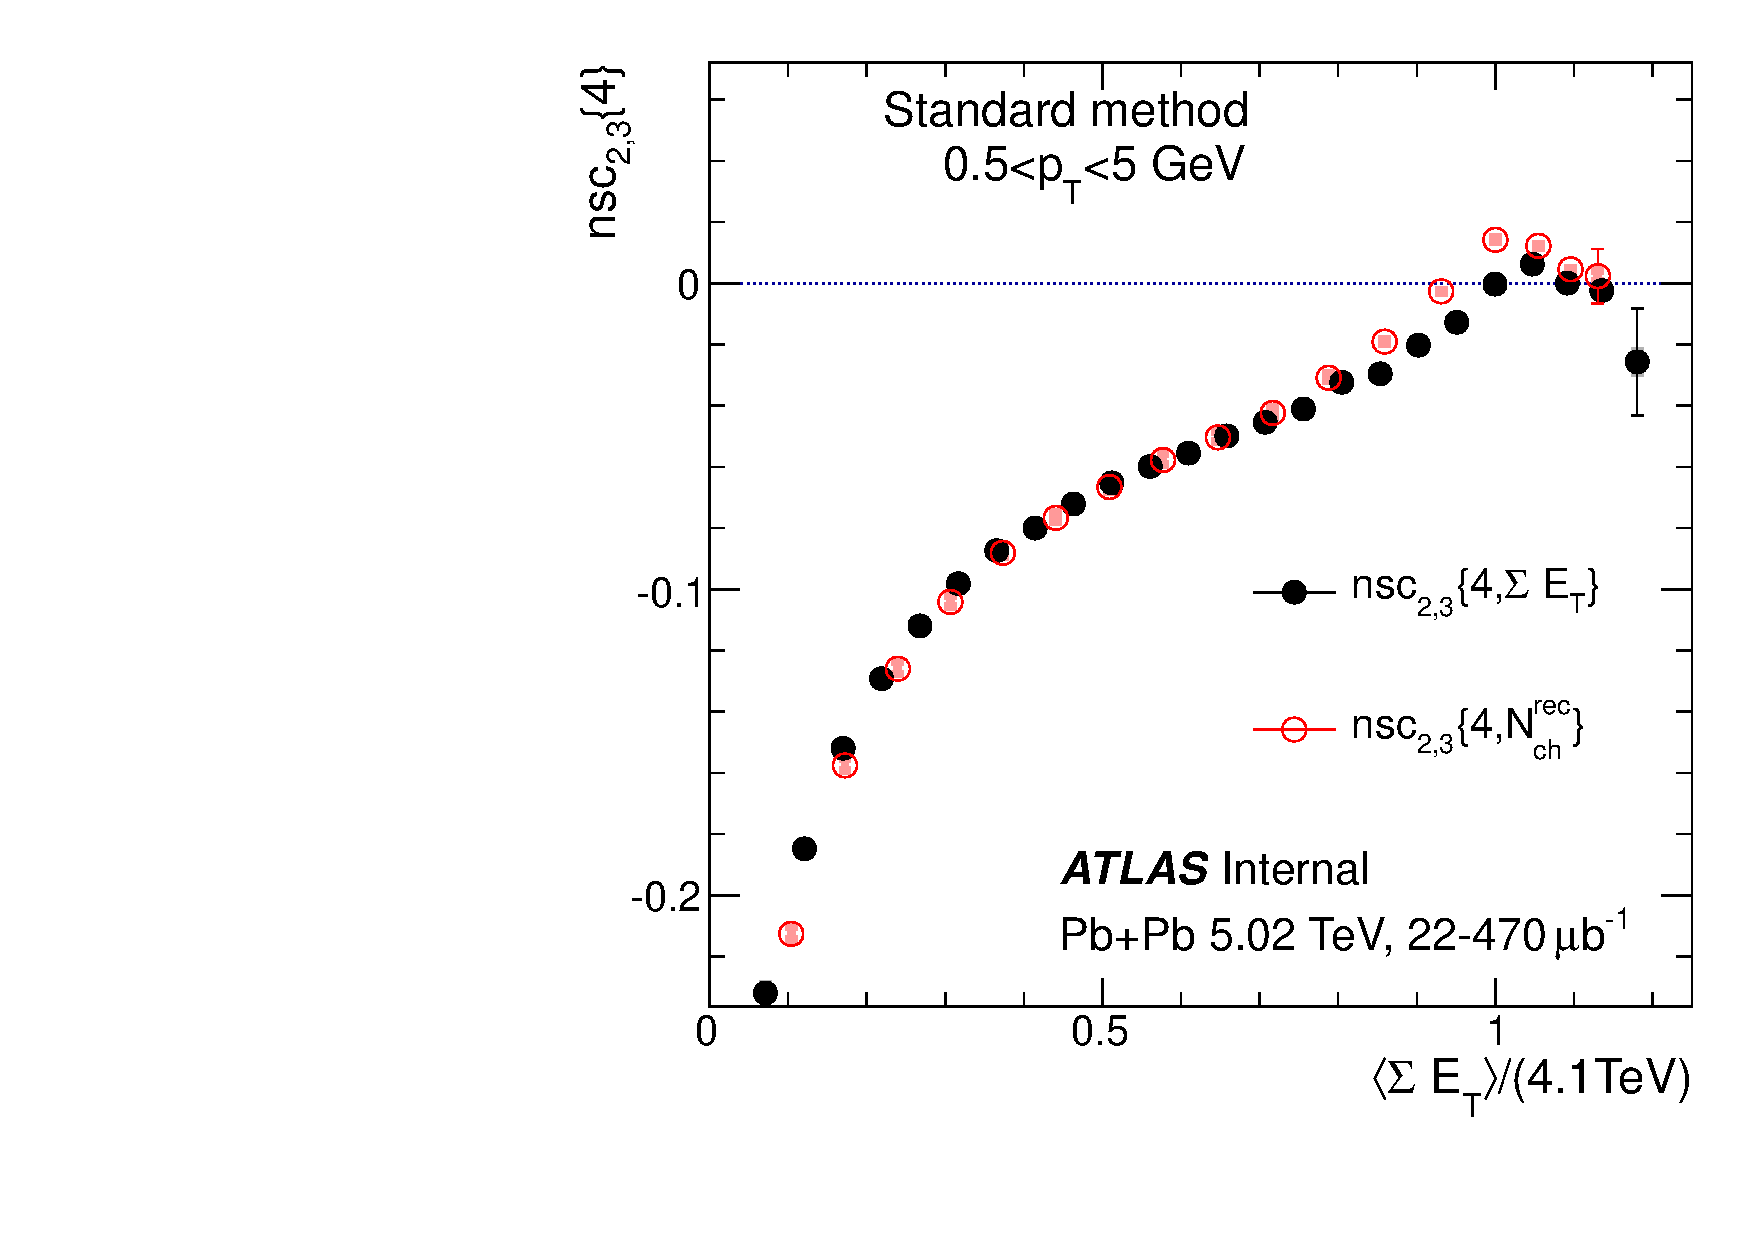
\includegraphics[width=.32\linewidth]{figs/sec_paper/comp_nsc_t0_har2_pt0.pdf}
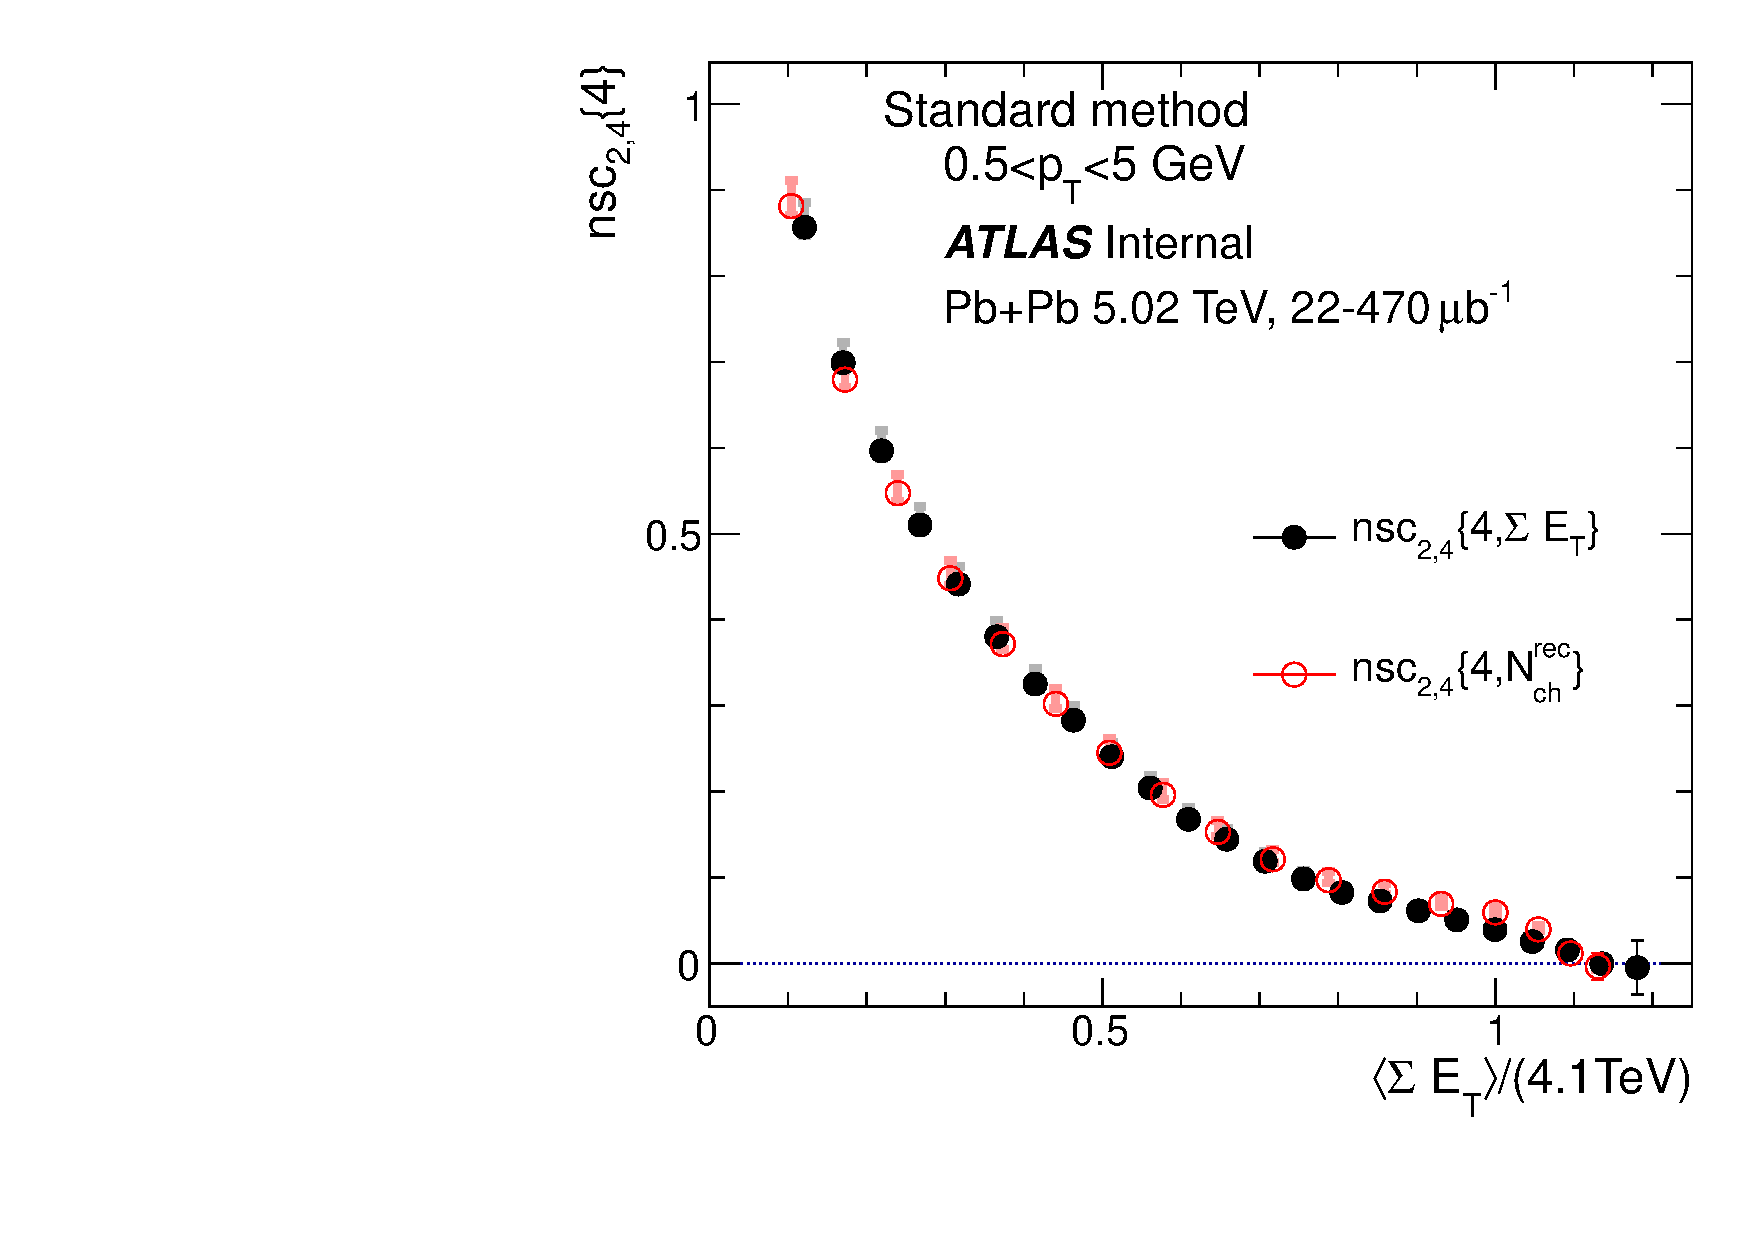
\includegraphics[width=.32\linewidth]{figs/sec_paper/comp_nsc_t0_har3_pt0.pdf}
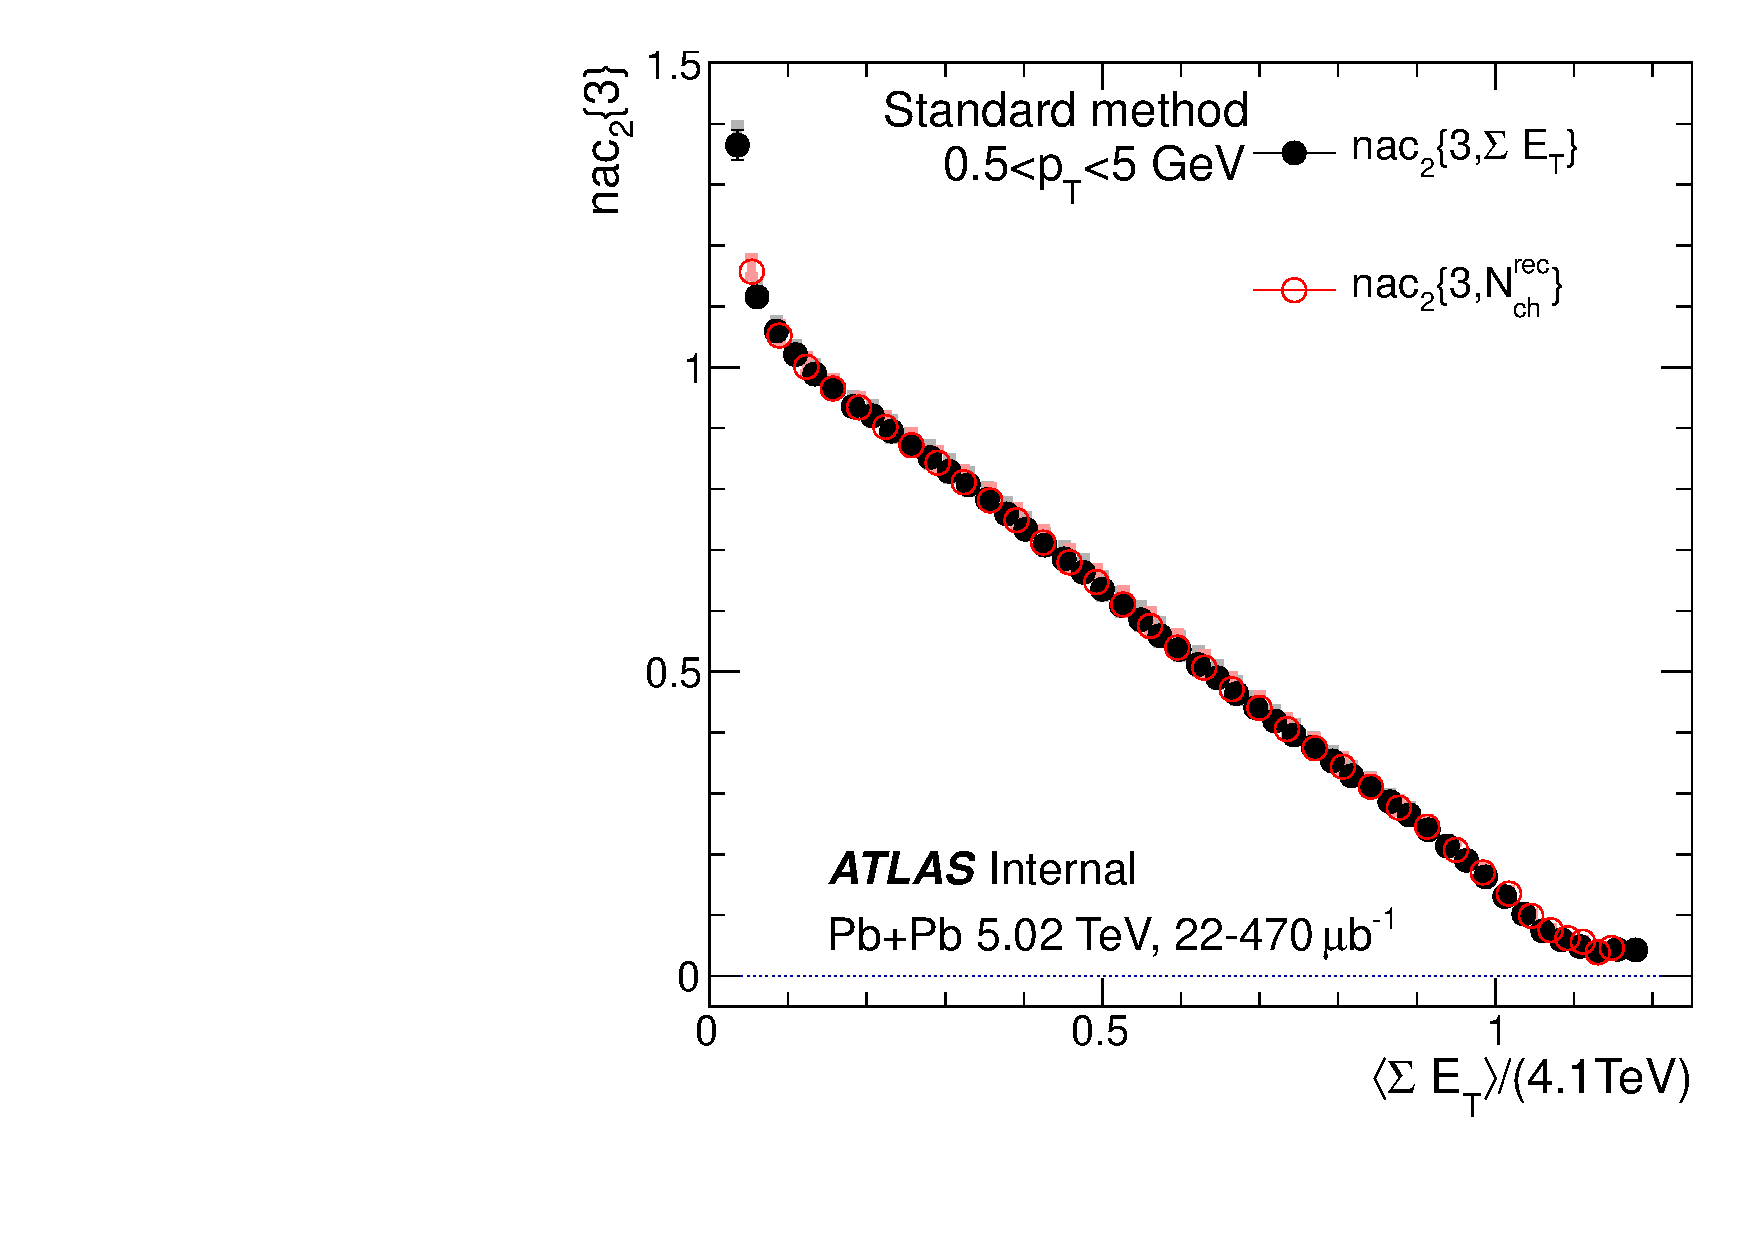
\includegraphics[width=.32\linewidth]{figs/sec_paper/comp_nac_t0_har2_pt0.pdf}
\caption{Check of volume fluctuation for symmetric and asymmetric cumulants.}
\label{fig:paper_vf_sc}
\end{figure}
